% --- Підрозділ 1 ---<<  >>
\section{Склад виробу}
У цьому розділі наводиться перелік основних компонентів конструктиву шасі <<SCHROFF 3U19>> та <<3U14,25>>.
\begin{table}[H]
    \centering
  \caption{Перелік деталей шасі}
    %\begin{tabular}{|p{1cm}|p{8cm}|p{3cm}|}
     \begin{tabular}{|p{0.8cm}|p{3.2cm}|p{7.5cm}|p{2cm}|} 
        \hline
        \textbf{№} & \textbf{№ за каталогом} & \textbf{Найменування} & \textbf{Кількість} \\ \hline
        1 & 34560-189 & Бічна панель EuropacPRO 3U19",295 мм. & 2 од. \\ \hline
        2 & 34560-184 & Рейка передня L-KD,84HP & 4 од. \\ \hline
        3 & 34560-163 & Рейка передня L-KD,63HP & 4 од. \\ \hline
        4 & 34560-484 & Рейка задня L-ST,84HP & 2 од. \\ \hline
        5 & 34560-463 & Рейка задня L-ST,63HP & 2 од. \\ \hline
        6 & 24560-197 & Кронштейн EuropacPRO,3U & 2 од. \\ \hline
        7 & 24561-198 & Профіль задній EuropacPRO,3U & 2 од. \\ \hline
        8 & 24560-080 & Панель верхня/нижня EuropacPRO, 295 мм,84HP & 2 од. \\ \hline
        9 & 24560-073 & Панель верхня/нижня EuropacPRO, 295 мм,63HP & 2 од. \\ \hline
       10 & 34561-484 & Планка різьбова М3х2х5 мм,84HP & 6 од. \\ \hline
       11 & 24560-235 & Планка контактна EuropacPRO EMC,84HP & 4 од. \\ \hline
       12 & 24560-233 & Планка контактна EuropacPRO EMC,63HP & 4 шт. \\ \hline
       13 & 21100-646 & Фіксатор планки різьбової,М3х8 мм & 12 од. \\ \hline
       14 & 24560-130 & Гвинт М4х14 мм, Torx & 12 од. \\ \hline
       15 & 24560-135 & Гвинт М4х6 мм, Torx & 32 од. \\ \hline
       16 & 24560-140 & Гайка квадратна, ступінчаста М4 & 13 од. \\ \hline
       17 & 34562-762 & Екран міжплатний EuropacPRO,3U,220 мм & Згідно специфікацій \\ \hline
       18 & 24560-353 & Напрямна для плат, 220 мм & Згідно специфікацій \\ \hline
       19 & ISO7380-2 & Гвинт М4х16 бурт. 10.9 цб INB & 1 од. \\ \hline
       20 & DIN6798A & Шайба 4 стопорна A4 зовнішні зубці & 1 од. \\ \hline
   
    \end{tabular}
    
\end{table}

\begin{figure}[H]
    \centering
    % Переконайтеся, що файл зображення завантажений в Overleaf
    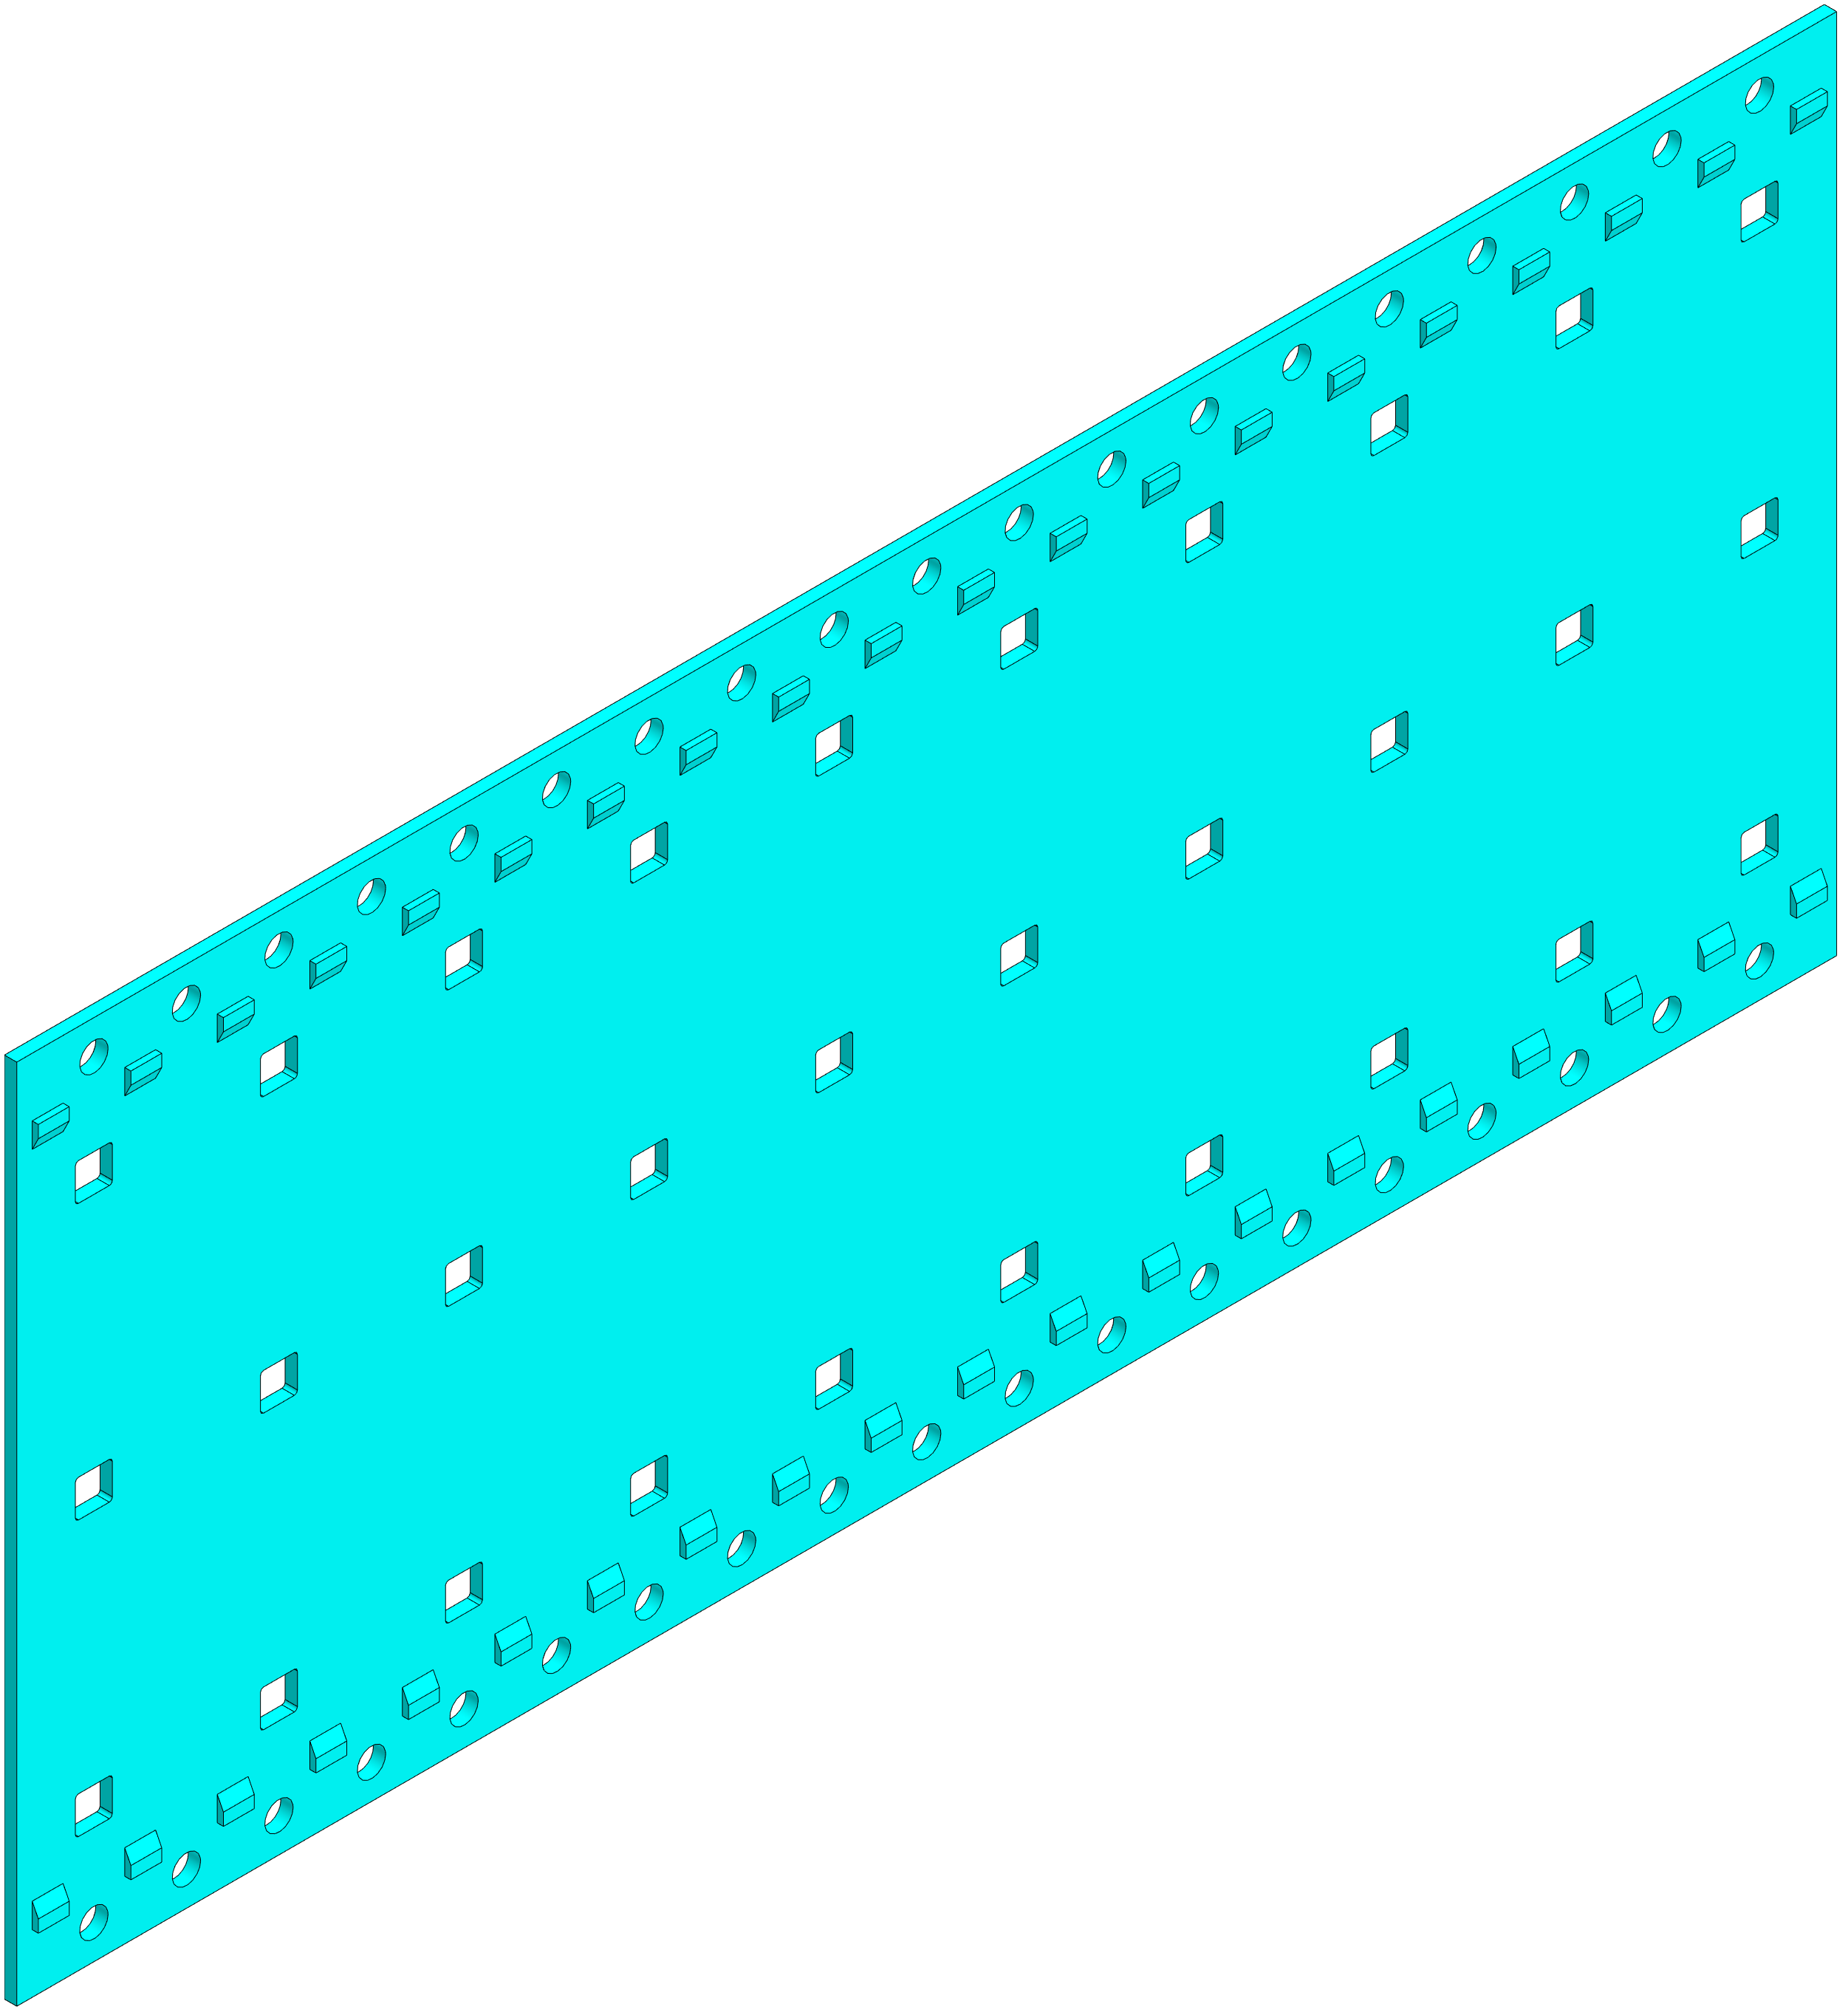
\includegraphics[width=0.7\textwidth]{images/A4.png} 
    \caption{Бічна панель EuropacPRO 3U19"}
\end{figure}

\begin{figure}[H]
    \centering
    % Переконайтеся, що файл зображення завантажений в Overleaf
    \includegraphics[width=0.9\textwidth]{images/A13.png} 
    \caption{Рейка передня L-KD,84HP}
\end{figure}

\begin{figure}[H]
    \centering
    % Переконайтеся, що файл зображення завантажений в Overleaf
    \includegraphics[width=0.75\textwidth]{images/A14.png} 
    \caption{Рейка передня L-KD,63HP}
\end{figure}

\begin{figure}[H]
    \centering
    % Переконайтеся, що файл зображення завантажений в Overleaf
    \includegraphics[width=0.75\textwidth]{images/A15.png} 
    \caption{Рейка задня L-ST,84HP}
\end{figure}

\begin{figure}[H]
    \centering
    % Переконайтеся, що файл зображення завантажений в Overleaf
    \includegraphics[width=0.75\textwidth]{images/A16.png} 
    \caption{Рейка задня L-ST,63HP}
\end{figure}

\begin{figure}[H]
    \centering
    % Переконайтеся, що файл зображення завантажений в Overleaf
    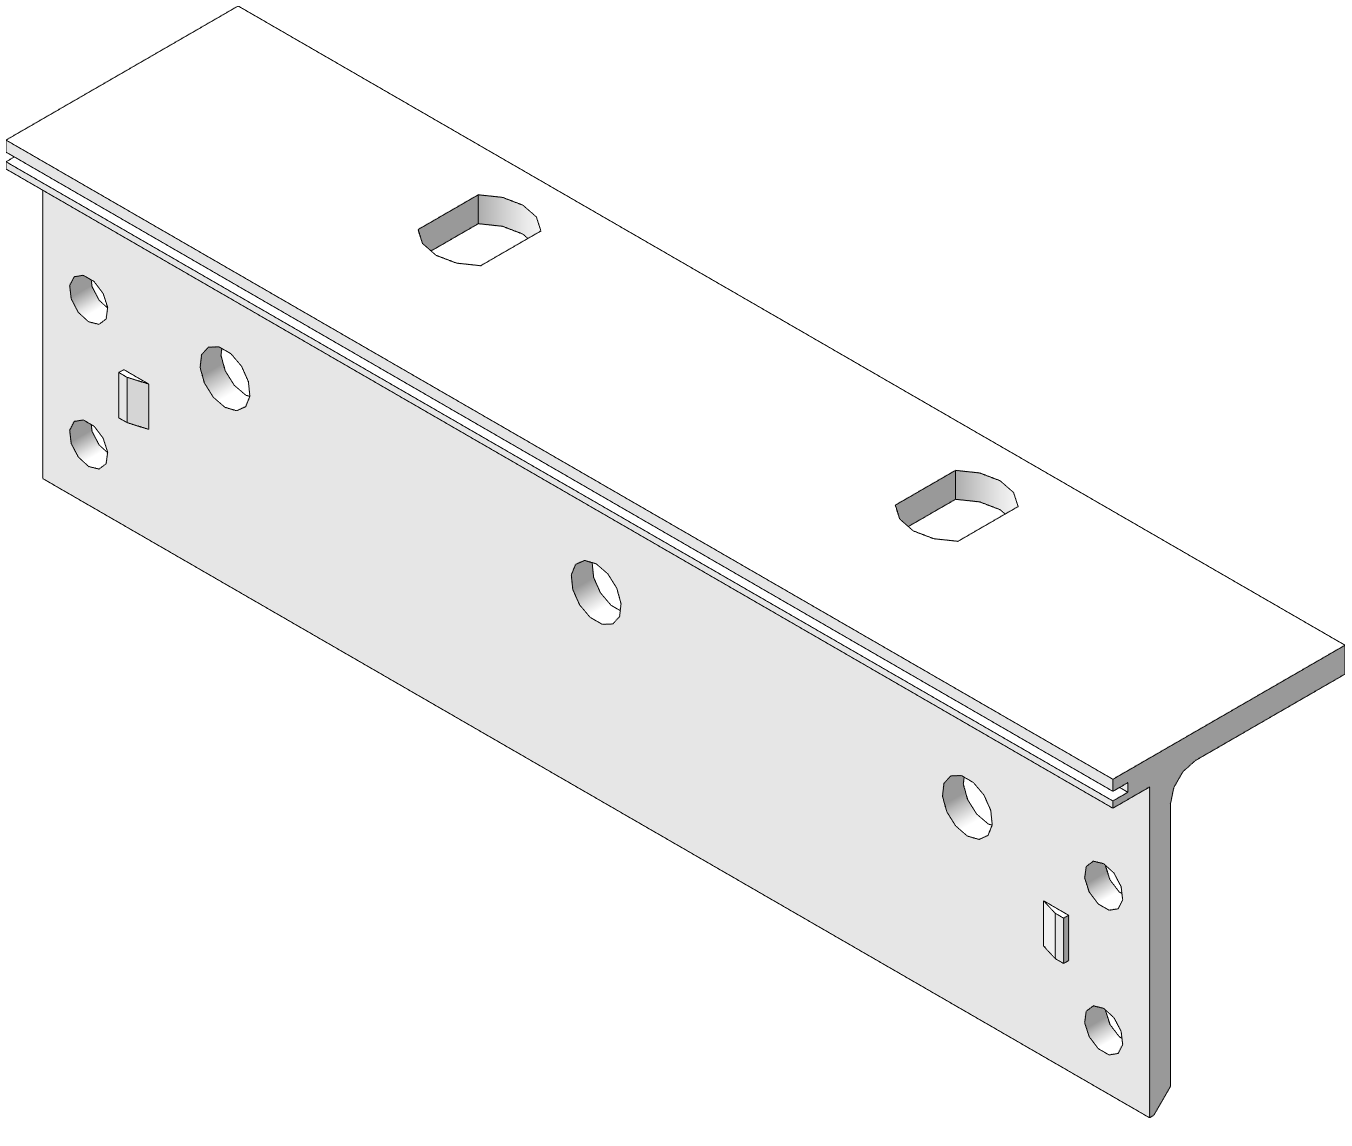
\includegraphics[width=0.5\textwidth]{images/A17.png} 
    \caption{Кронштейн EuropacPRO,3U}
\end{figure}

\begin{figure}[H]
    \centering
    % Переконайтеся, що файл зображення завантажений в Overleaf
    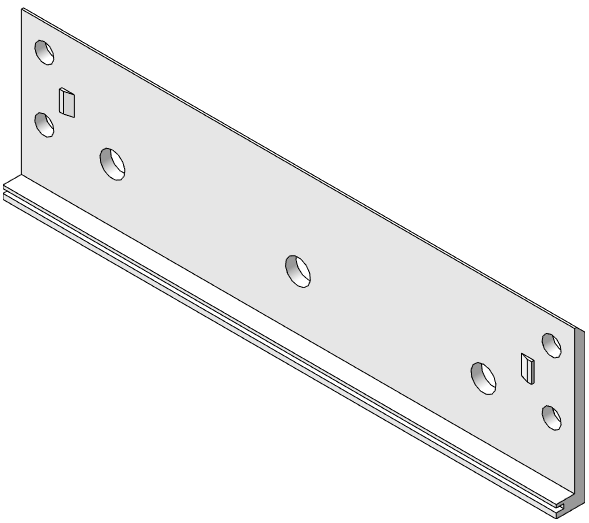
\includegraphics[width=0.5\textwidth]{images/A18.png} 
    \caption{Профіль задній EuropacPRO,3U}
\end{figure}

\begin{figure}[H]
    \centering
    % Переконайтеся, що файл зображення завантажений в Overleaf
    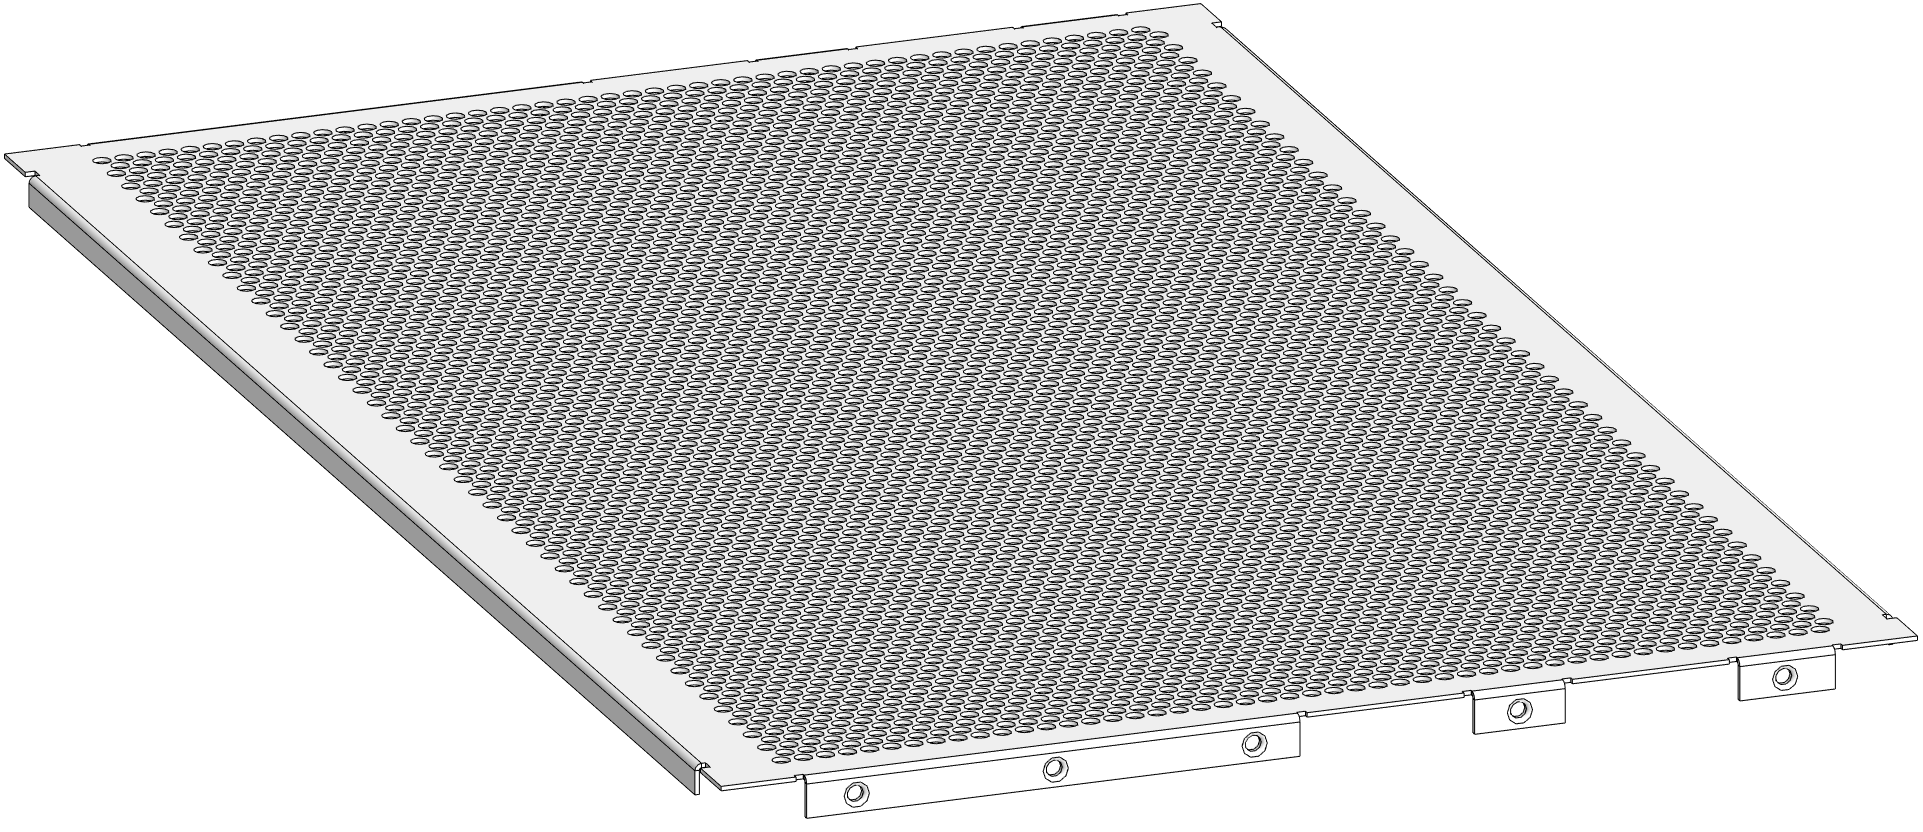
\includegraphics[width=0.5\textwidth]{images/A19.png} 
    \caption{Панель верхня/нижня EuropacPRO, 295 мм,84HP}
\end{figure}

\begin{figure}[H]
    \centering
    % Переконайтеся, що файл зображення завантажений в Overleaf
    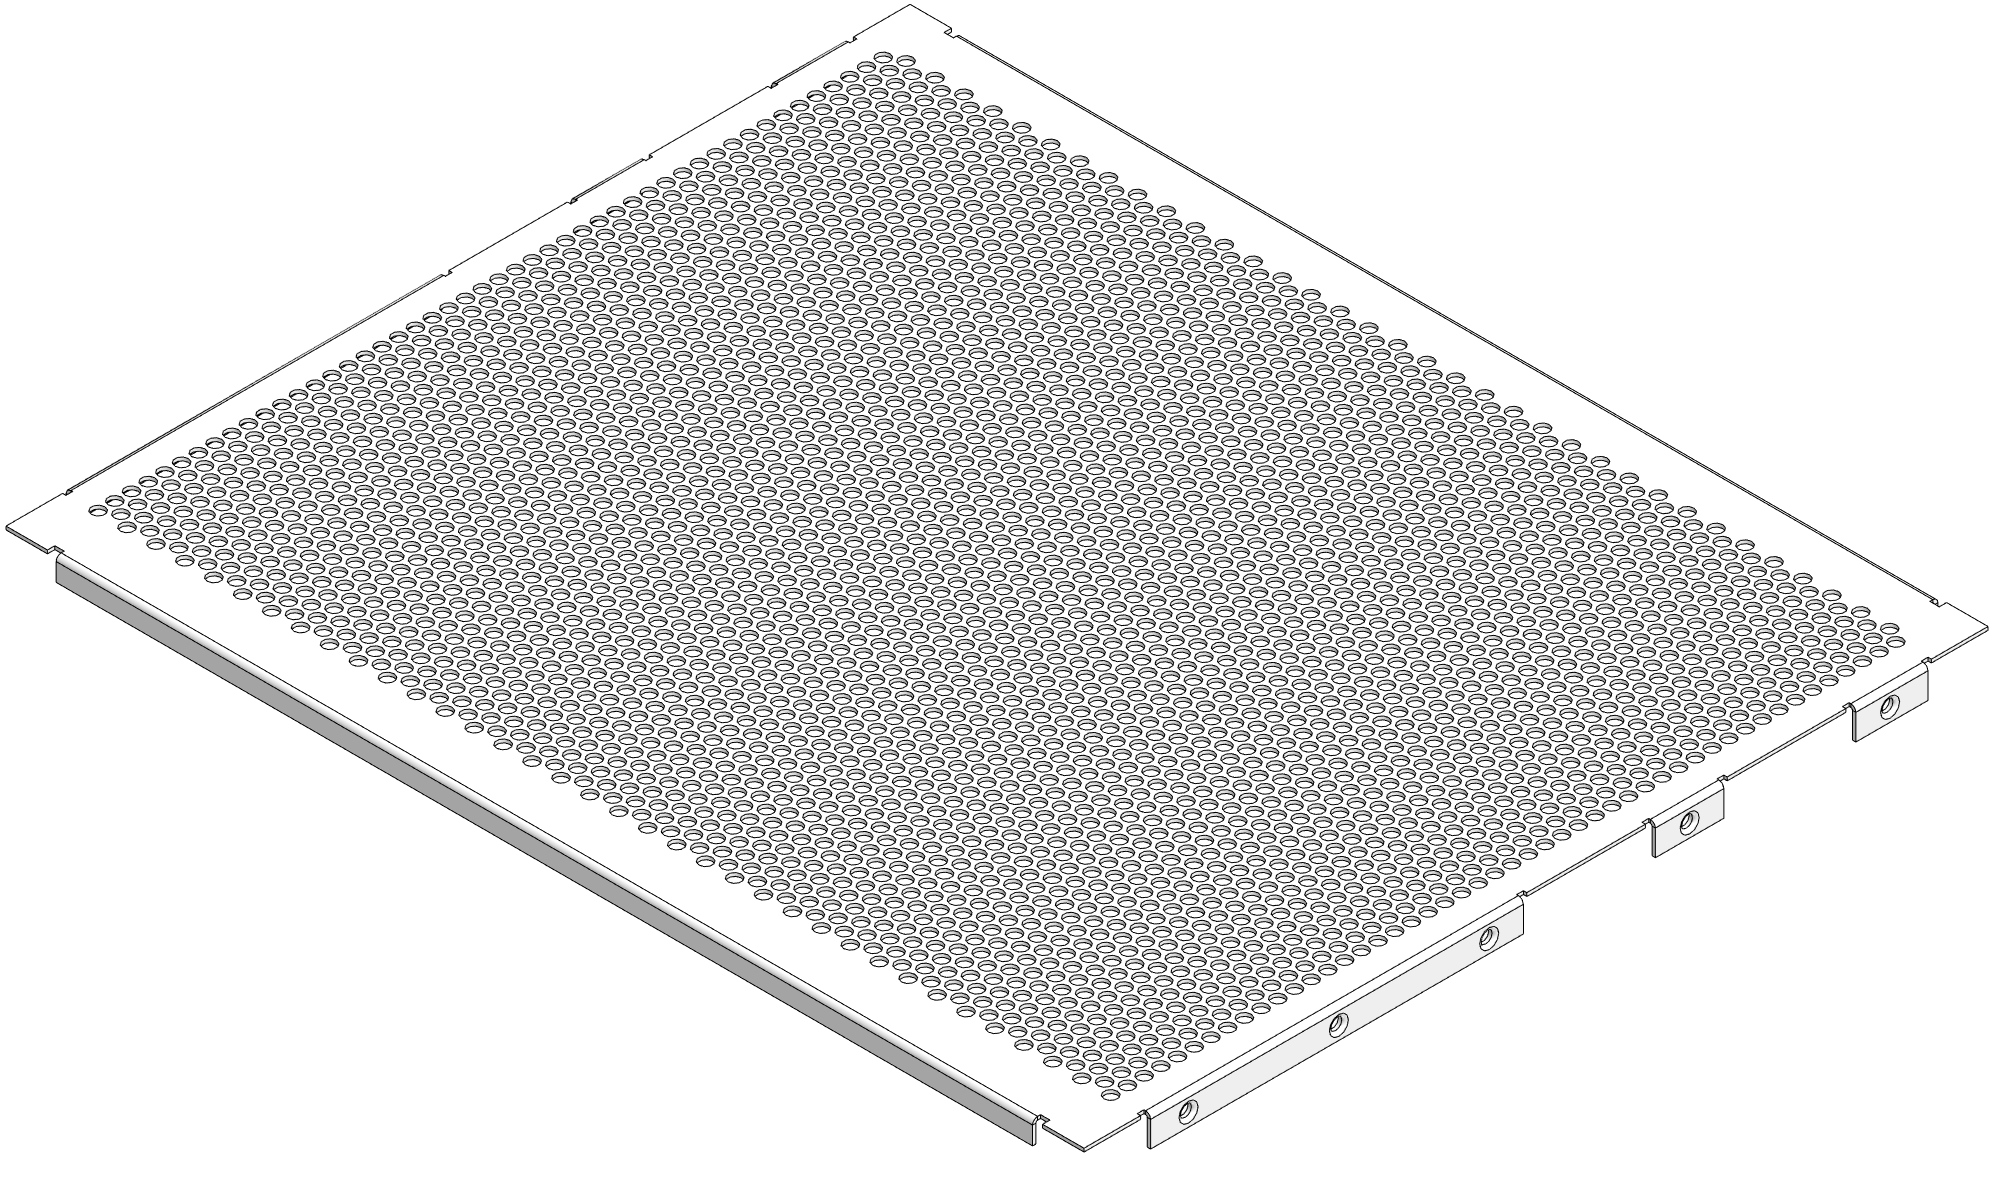
\includegraphics[width=0.5\textwidth]{images/A20.png} 
    \caption{Панель верхня/нижня EuropacPRO, 295 мм,63HP}
\end{figure}

\begin{figure}[H]
    \centering
    % Переконайтеся, що файл зображення завантажений в Overleaf
    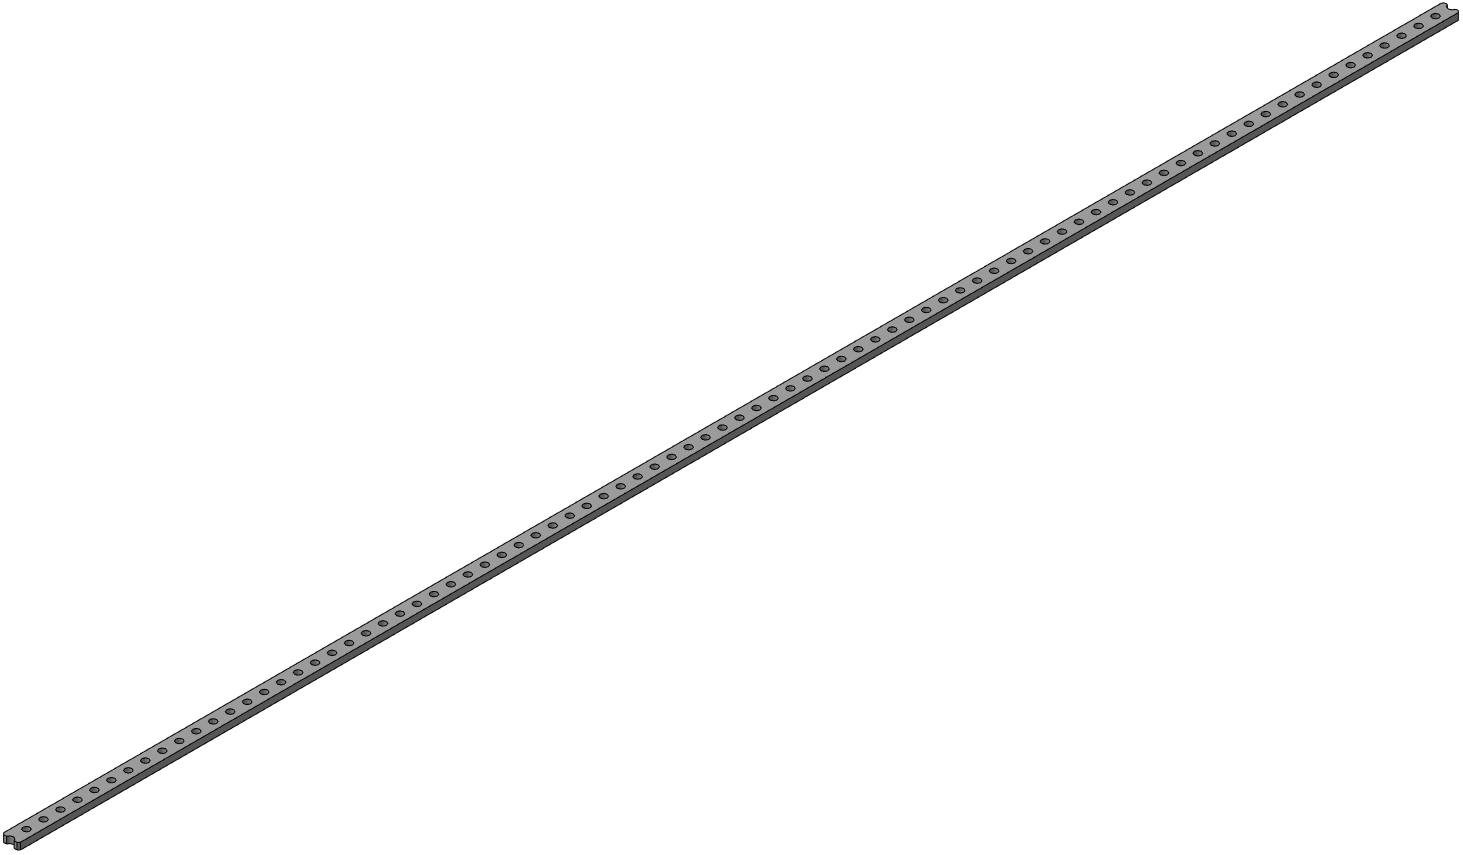
\includegraphics[width=0.5\textwidth]{images/A21.png} 
    \caption{Планка різьбова М3х2х5 мм,84HP}
\end{figure}

\begin{figure}[H]
    \centering
    % Переконайтеся, що файл зображення завантажений в Overleaf
    
\includegraphics[width=0.9\textwidth]{images/A22.png} 
    \caption{Планка контактна EuropacPRO EMC,84HP}
\end{figure}

\begin{figure}[H]
    \centering
    % Переконайтеся, що файл зображення завантажений в Overleaf
    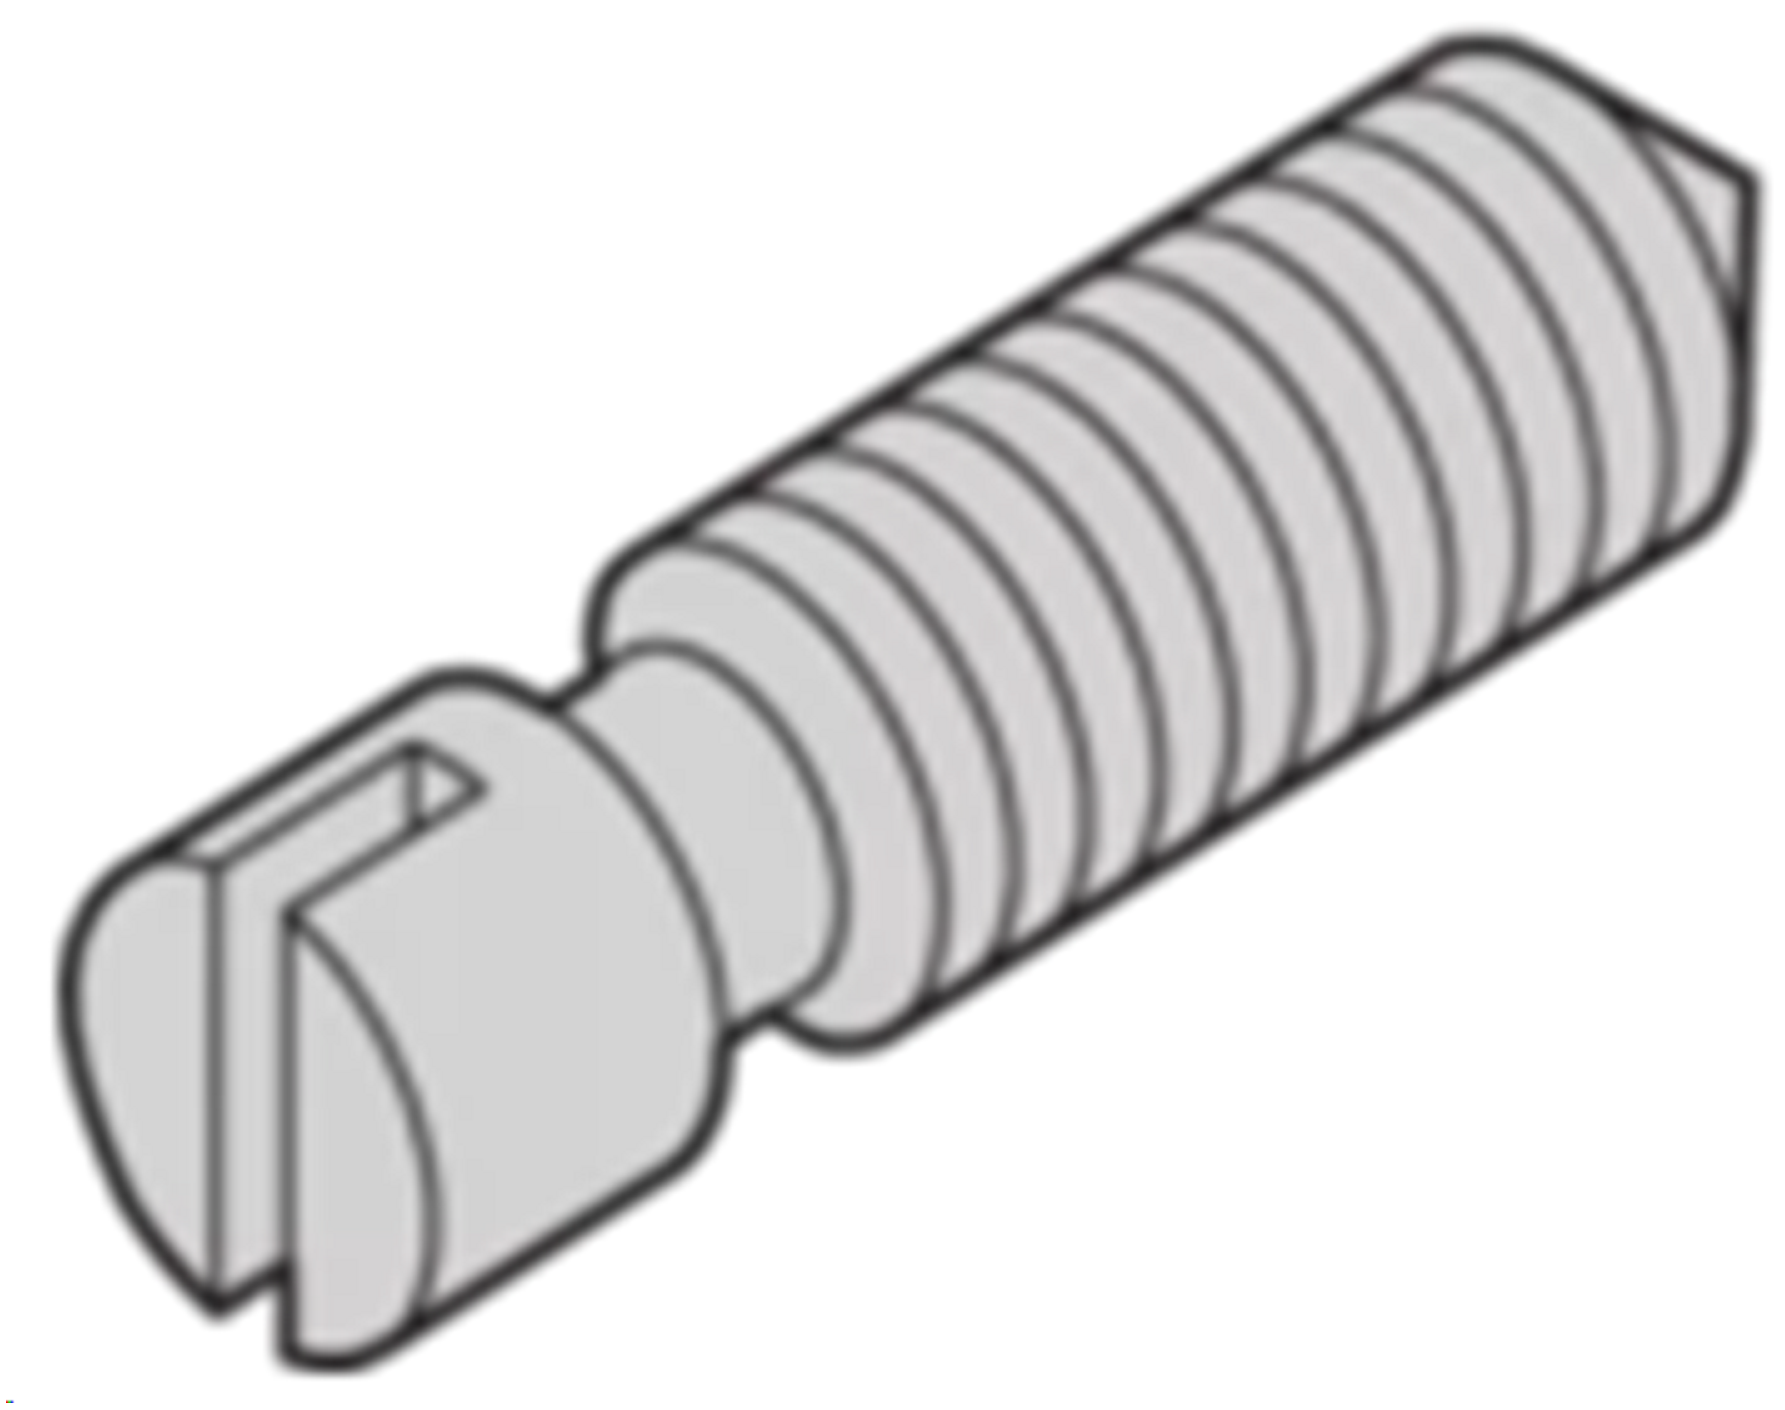
\includegraphics[width=0.25\textwidth]{images/A23.png} 
    \caption{Фіксатор планки різьбової,М3х8}
\end{figure}

\begin{figure}[H]
    \centering
    % Переконайтеся, що файл зображення завантажений в Overleaf
    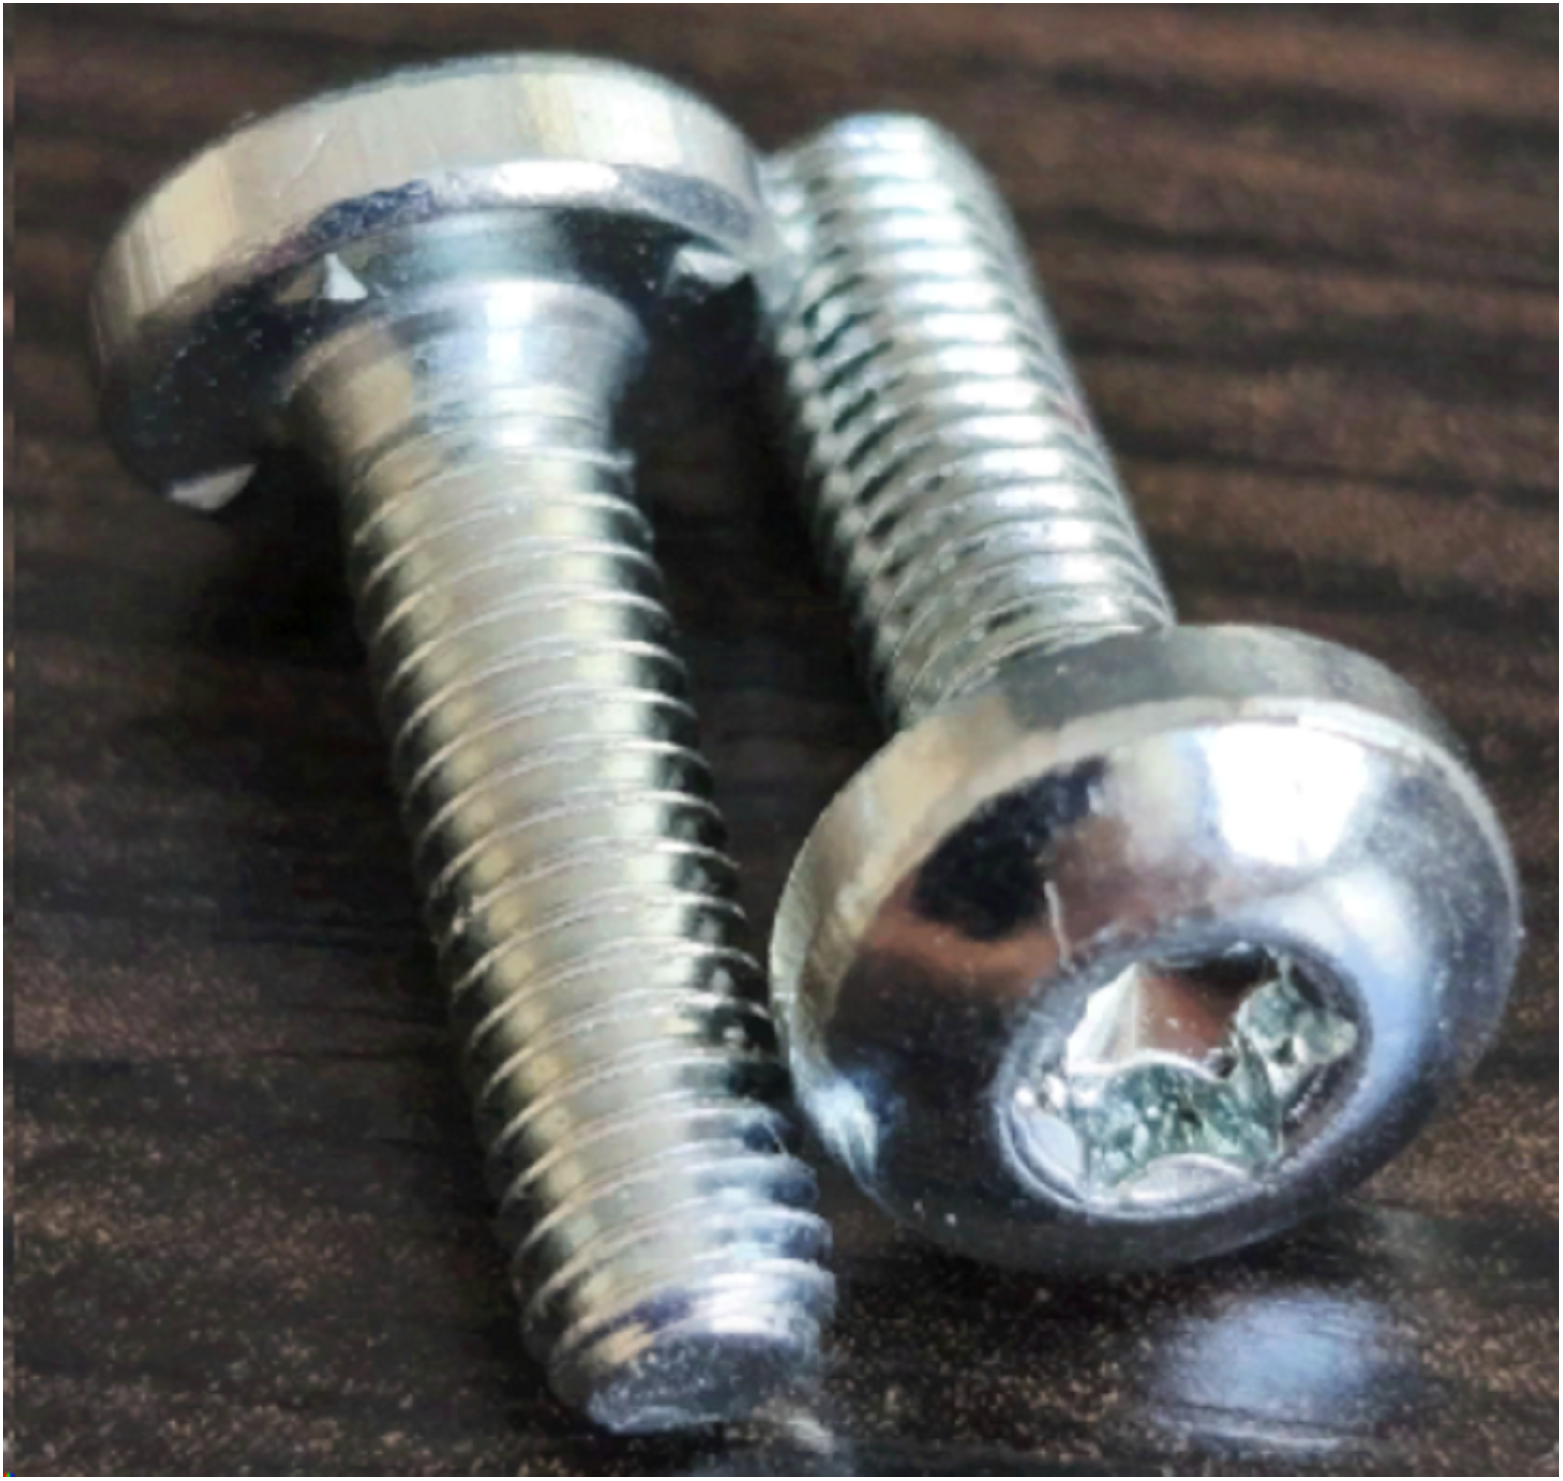
\includegraphics[width=0.35\textwidth]{images/A24.png} 
    \caption{Гвинт М4х14 мм, Torx}
\end{figure}

\begin{figure}[H]
    \centering
    % Переконайтеся, що файл зображення завантажений в Overleaf
    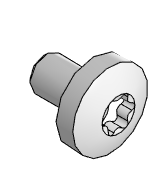
\includegraphics[width=0.4\textwidth]{images/A25.png} 
    \caption{Гвинт М4х6 мм, Torx}
\end{figure}

\begin{figure}[H]
    \centering
    % Переконайтеся, що файл зображення завантажений в Overleaf
    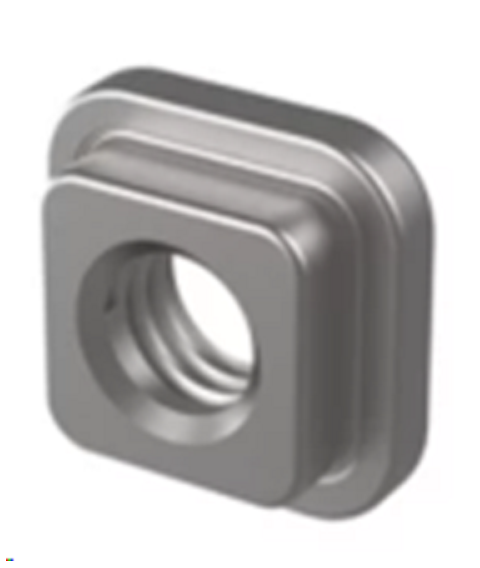
\includegraphics[width=0.25\textwidth]{images/A26.png} 
    \caption{Гайка квадратна, ступінчаста М4}
\end{figure}

\begin{figure}[H]
    \centering
    % Переконайтеся, що файл зображення завантажений в Overleaf
    \includegraphics[width=0.75\textwidth]{images/A33.pdf} 
    \caption{Екран міжплатний EuropacPRO,3U,220 мм}
\end{figure}

\begin{figure}[H]
    \centering
    % Переконайтеся, що файл зображення завантажений в Overleaf
    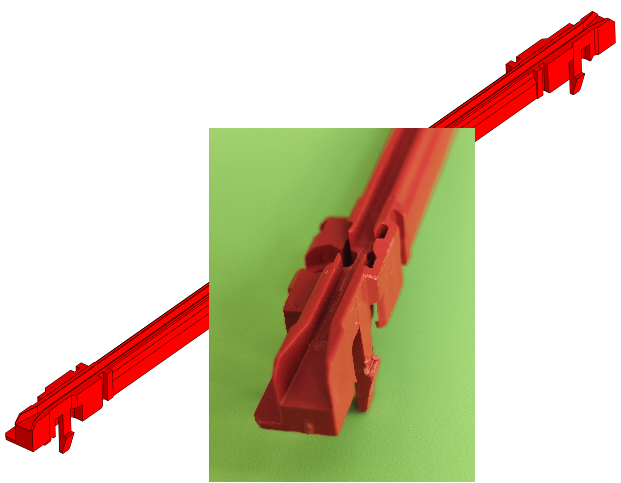
\includegraphics[width=0.75\textwidth]{images/A34.png} 
    \caption{Напрямна для плат, 220 мм}
\end{figure}

\begin{figure}[H]
    \centering
    % Переконайтеся, що файл зображення завантажений в Overleaf
    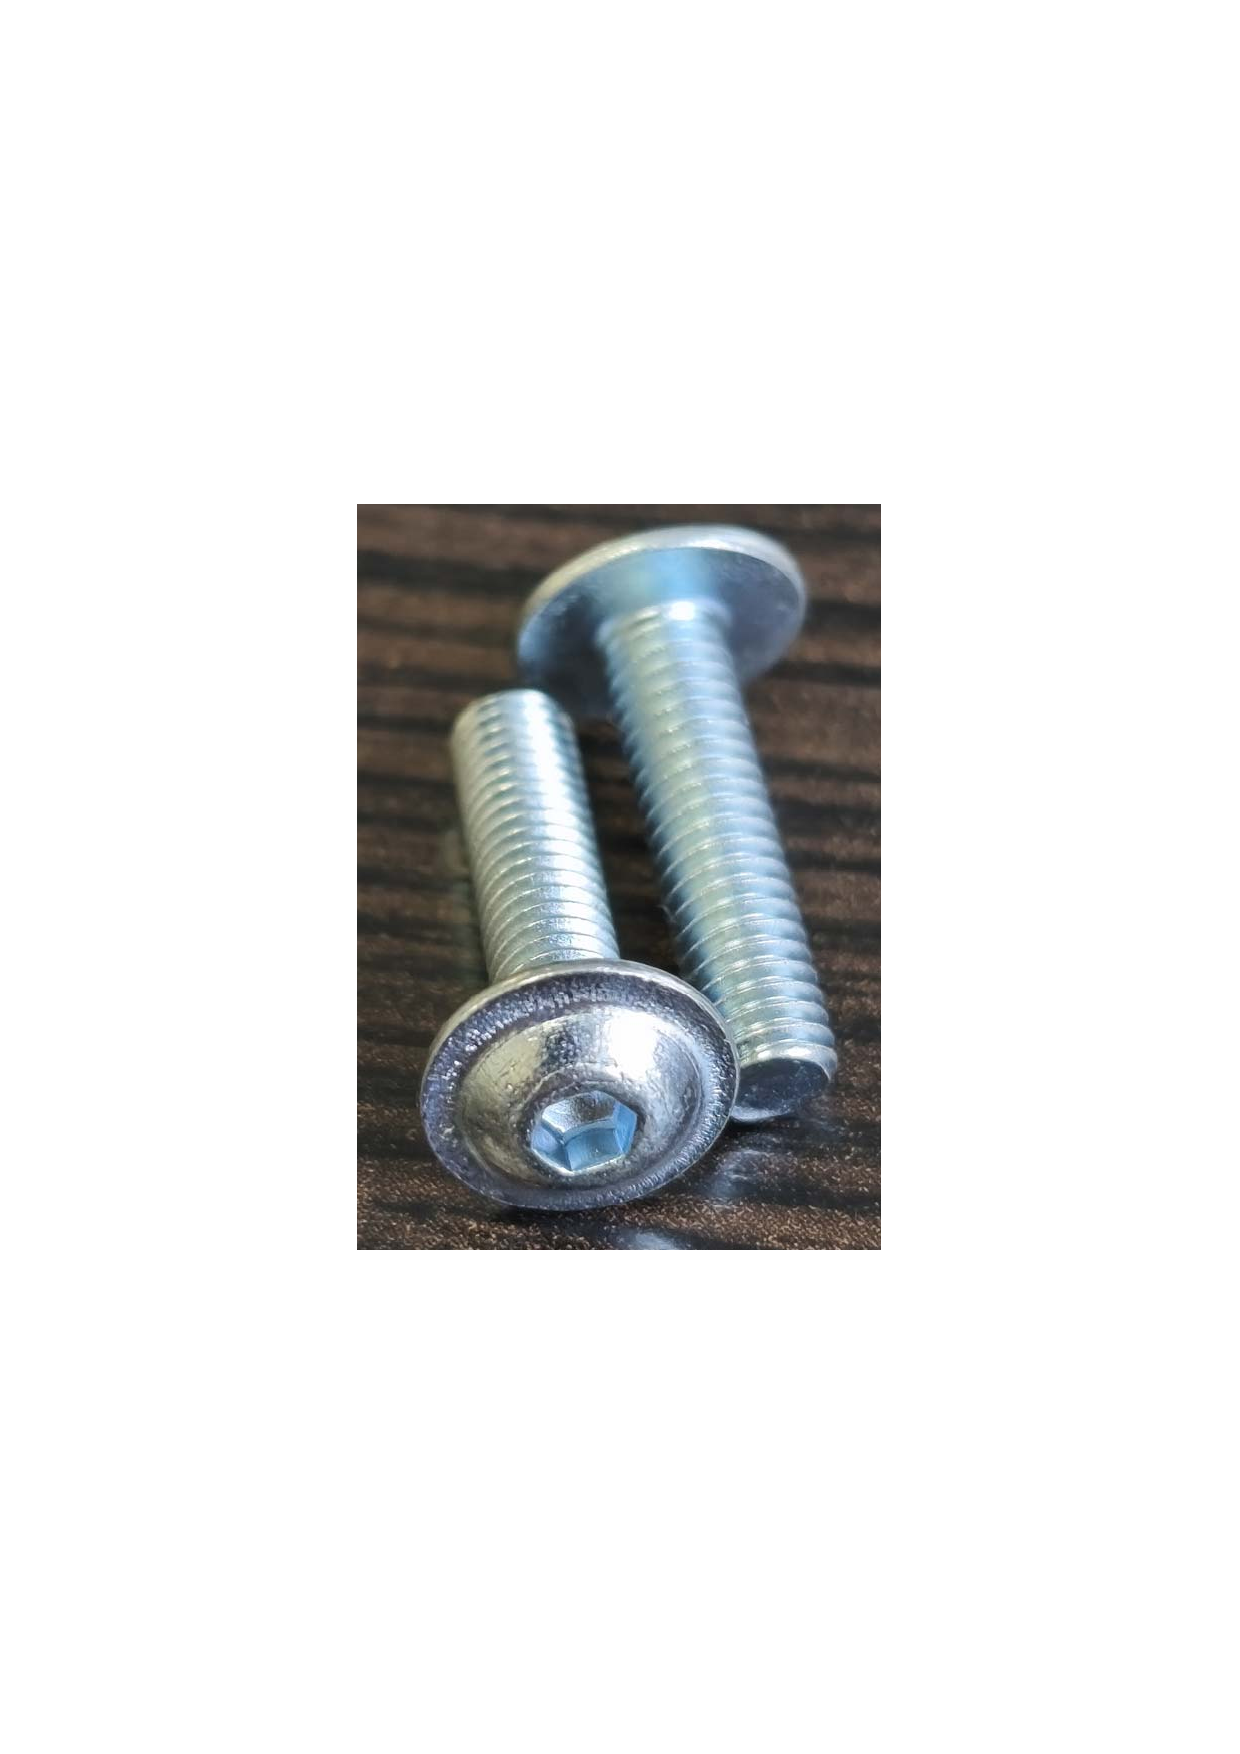
\includegraphics[width=0.25\textwidth]{images/A45.pdf} 
    \caption{Гвинт М4х16 бурт. 10.9 цб INB}
\end{figure}

\begin{figure}[H]
    \centering
    % Переконайтеся, що файл зображення завантажений в Overleaf
    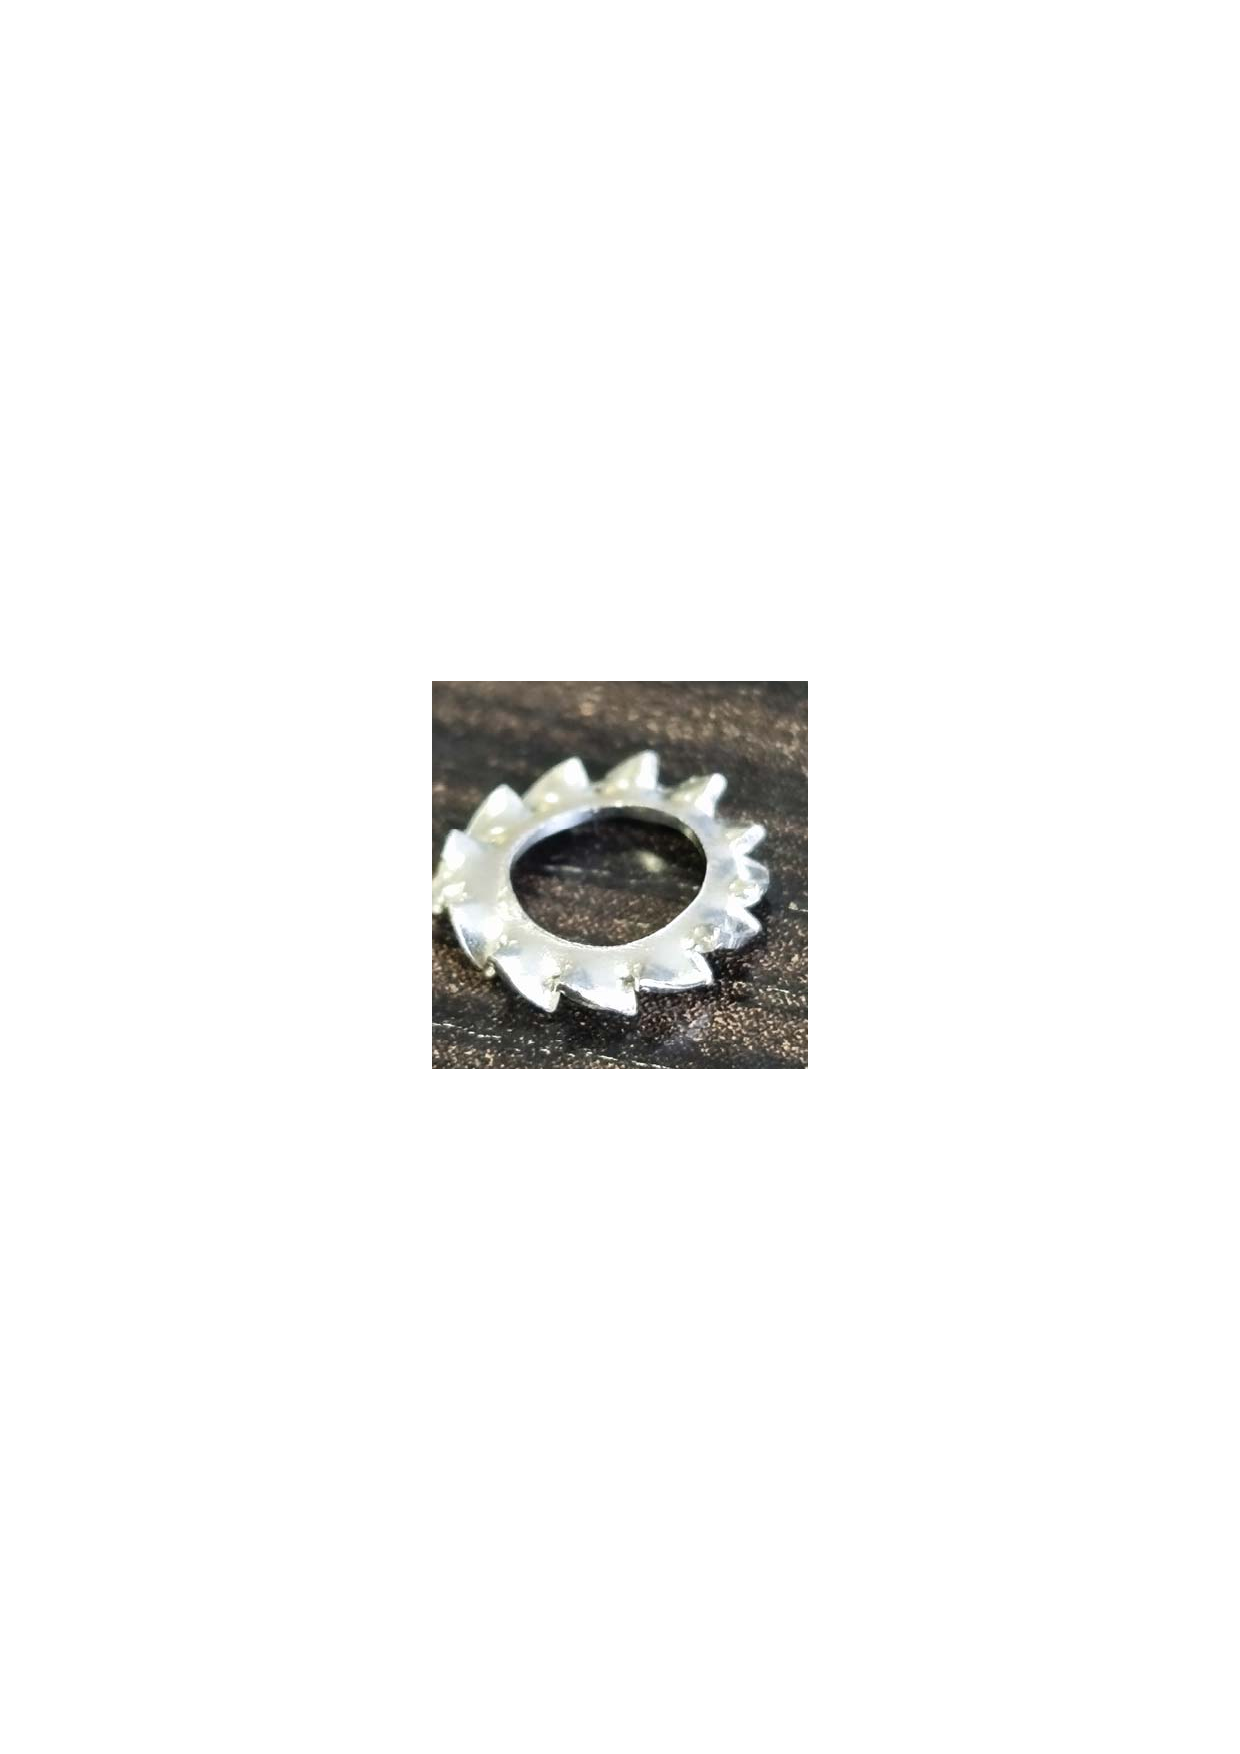
\includegraphics[width=0.45\textwidth]{images/A44.pdf} 
    \caption{Шайба 4 стопорна A4 зовнішні зубці}
\end{figure}


\newpage

% --- Підрозділ 2 ---
\section{Технологічні вимоги до процесу складання корпусів}
\subsection{Організація робочого місця та місця зберігання}
Складання конструктиву шасі треба виконувати на плоскій твердій поверхні, яка з метою унеможливлення механічних пошкоджень деталей має бути вкрита
агроволокном білого кольору, спанбондом, щільністю 100 гр/м2. Ширина поверхні для складання має бути 0,8 м, довжина не менше 1,5 м, висота над равнем
підлоги 0,7-0,75 м.

З метою зберігання товарного зовнішнього вигляду та уникнення механічних ушкоджень конструктиву корпусів, процесс їхнього складання та зберігання має відбуватися з використанням тонких, чистих, бавовняних рукавичок з антислизовим малюнком. На рукавичках мають бути відсутні плями бруду та жиру. 

З метою уникнення механічних ушкоджень на конструктиві корпусів у процесі складання та зберігання, забезпечити розміщення складових таким чином щоб унеможливити їх механічний контакт на місці складання за допомогою використання органайзерів для окремих видів деталей. 

Конструктив шасі корпусу скріплюється з використанням самофіксуючих гвинтів М4х14 та М4х6 TORX, а також ступінчастих квадратних гайок М4. Процесс збирання здійснюється з використанням динамометричних викруток та біт Т15-Т20(TORX). Моменти затягування гвинтів наведено у розділі 3 <<Порядок складання>>.

Зібрані та готові до використання конструктиви шасі мають бути промарковані. Маркування має включати:
- дату складання з 6-ох цифр(число,місяць,рік),
- тризначний номер що позначає тип приладу який має складатися з використання саме цього конструктиву,
- номер що ідентифікує особу яка робила складання конструктиву.

Маркування пишеться в рядок у вигляді 3 груп цифр через проміжок(ХХХХХХ-ХХХ-ХХХ).

Маркування робиться на стікері що клеїться на внутрішній площині правої бокової стінки у передній частині на середині висоти конструктиву.  

Після маркування конструктив має бути обгорнутим у стрейч-плівку, якщо не передбачається його негайне використання у подальшому технологічному процесі.
Забороняється в процесі зберігання класти конструктиви один на одний без використання проміжного шару спанбонду. Висота штабелювання не більше 5 одиниць. 

\subsection{Позиціювання конструктиву та його складових}

\begin{figure}[H]
    \centering
    % Переконайтеся, що файл зображення завантажений в Overleaf
    \includegraphics[width=1.0\textwidth]{images/A28.png} 
    \caption{Схема позиціонування складових шасі 3U19"}
\end{figure}

На малюнку 1.20 зображено конструктив шасі <<ВИД ЗЗАДУ>> з одночасним суміщенням розгорнутих на 90 градусів верхньої та нижньої << Рейок передніх L-KD,84HP>>. 

Рейки суміщені та разгорнуті таким чином, що видно цифрову розмітку. Розмітка співпадає з реальним позиціюванням рейок відносно конструктиву шасі у горизонтальній площині. 

Надалі місця розташування <<Напрямних для плат>> та <<Екранів міжплатних EuropacPRO>> буде вказуватися як зображено на малюнку 1.20 тобто ЗЛІВА-НАПРАВО, починаючи з лівого, нижнього кута задньої площини конструктиву шасі. На <<Нижній передній рейці LK-D,84HP>> це відповідає отвору №1.

Місце розташування <<Напрямних для плат>> та <<Екранів міжплатних EuropacPRO>> позначається сукупністю двох чисел через скісну риску(слеш). Число ліворуч від риски, це номер по порядку згідно Мал.1.20. Число праворуч від риски, це номер отвору на <<Рейці передній L-KD,84HP>>(<<Рейці передній L-KD,63HP>>) куди вставляється відповідна ніжка <<Напрямної>>(Мал.1.20 та 1.23) або ніжки <<Екранів міжплатних>>(Мал.1.20). 

Приклад позначення:<<Напрямна ХХ/ХХ>>, <<Екран міжплатний ХХ/ХХ>>, або <<Напрямні: ХХ/ХХ, ХХ/ХХ...(перелік масиву)>>. Теж саме для <<Екранів міжплатних>>.

\begin{figure}[H]


    \centering
    % Переконайтеся, що файл зображення завантажений в Overleaf
    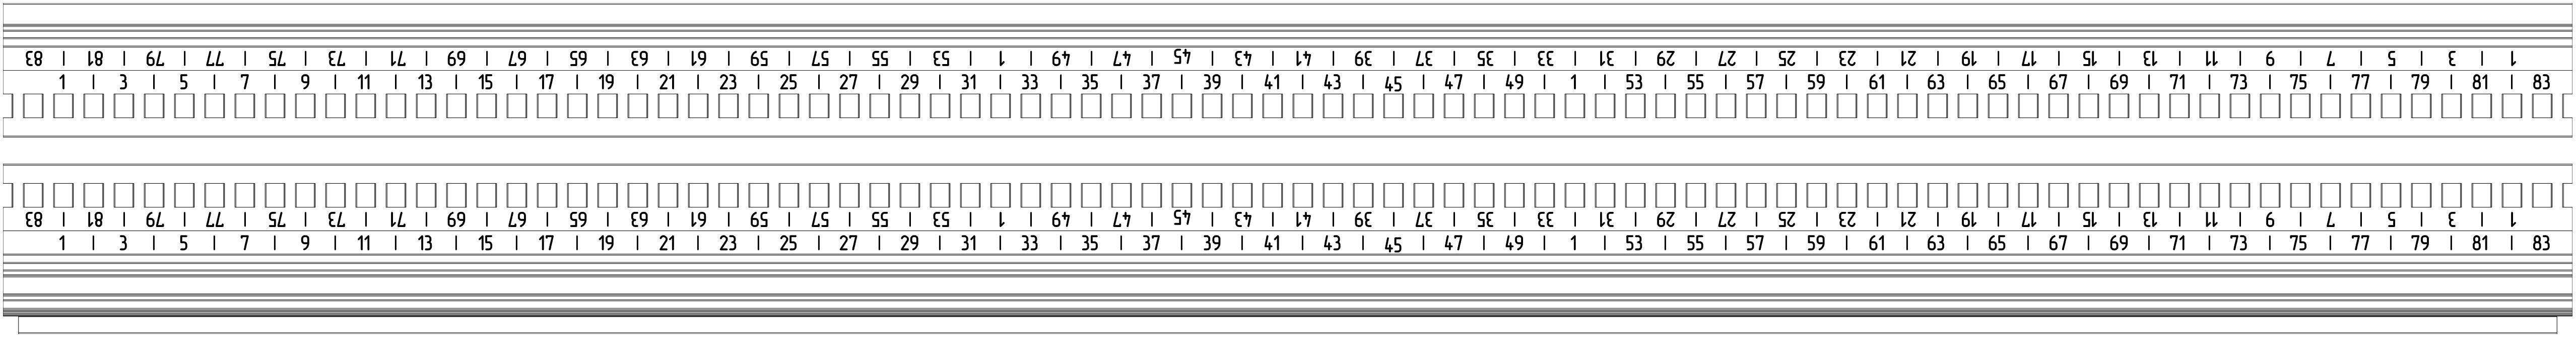
\includegraphics[width=1.0\textwidth]{images/A29.png} 
    \caption{Схема позиціонування передньої та задньої рейок 84HP}
\end{figure}


\begin{figure}[H]
    \centering
    % Переконайтеся, що файл зображення завантажений в Overleaf
    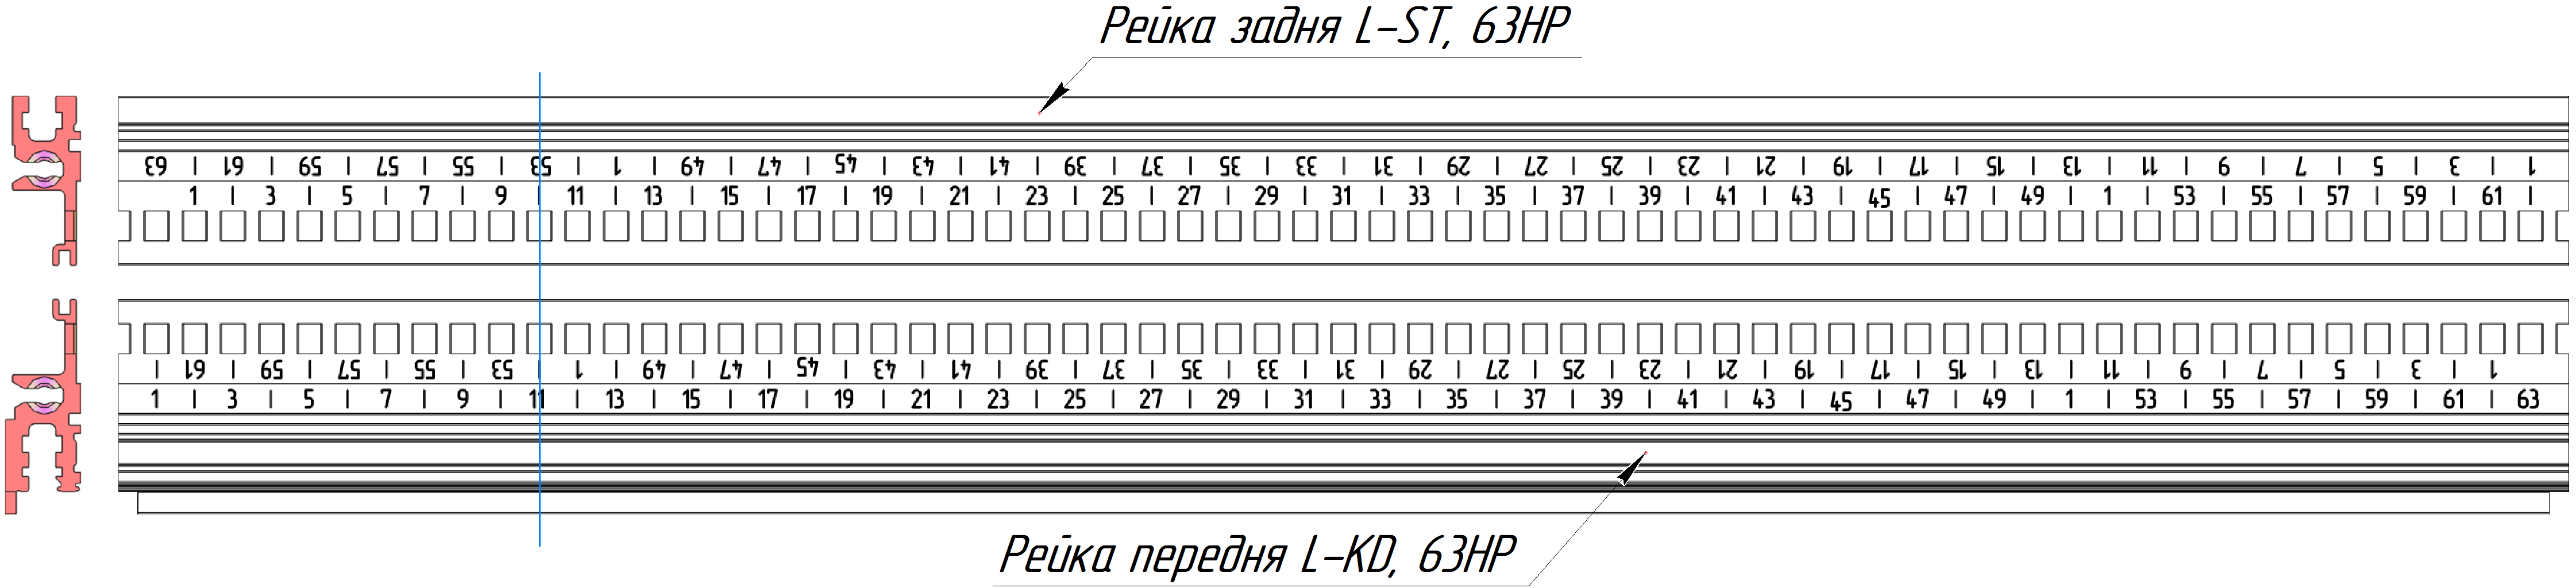
\includegraphics[width=1.0\textwidth]{images/A31.png} 
    \caption{Схема позиціонування передньої та задньої рейок 63HP}
\end{figure}


\begin{figure}[H]
    \centering
    % Переконайтеся, що файл зображення завантажений в Overleaf
    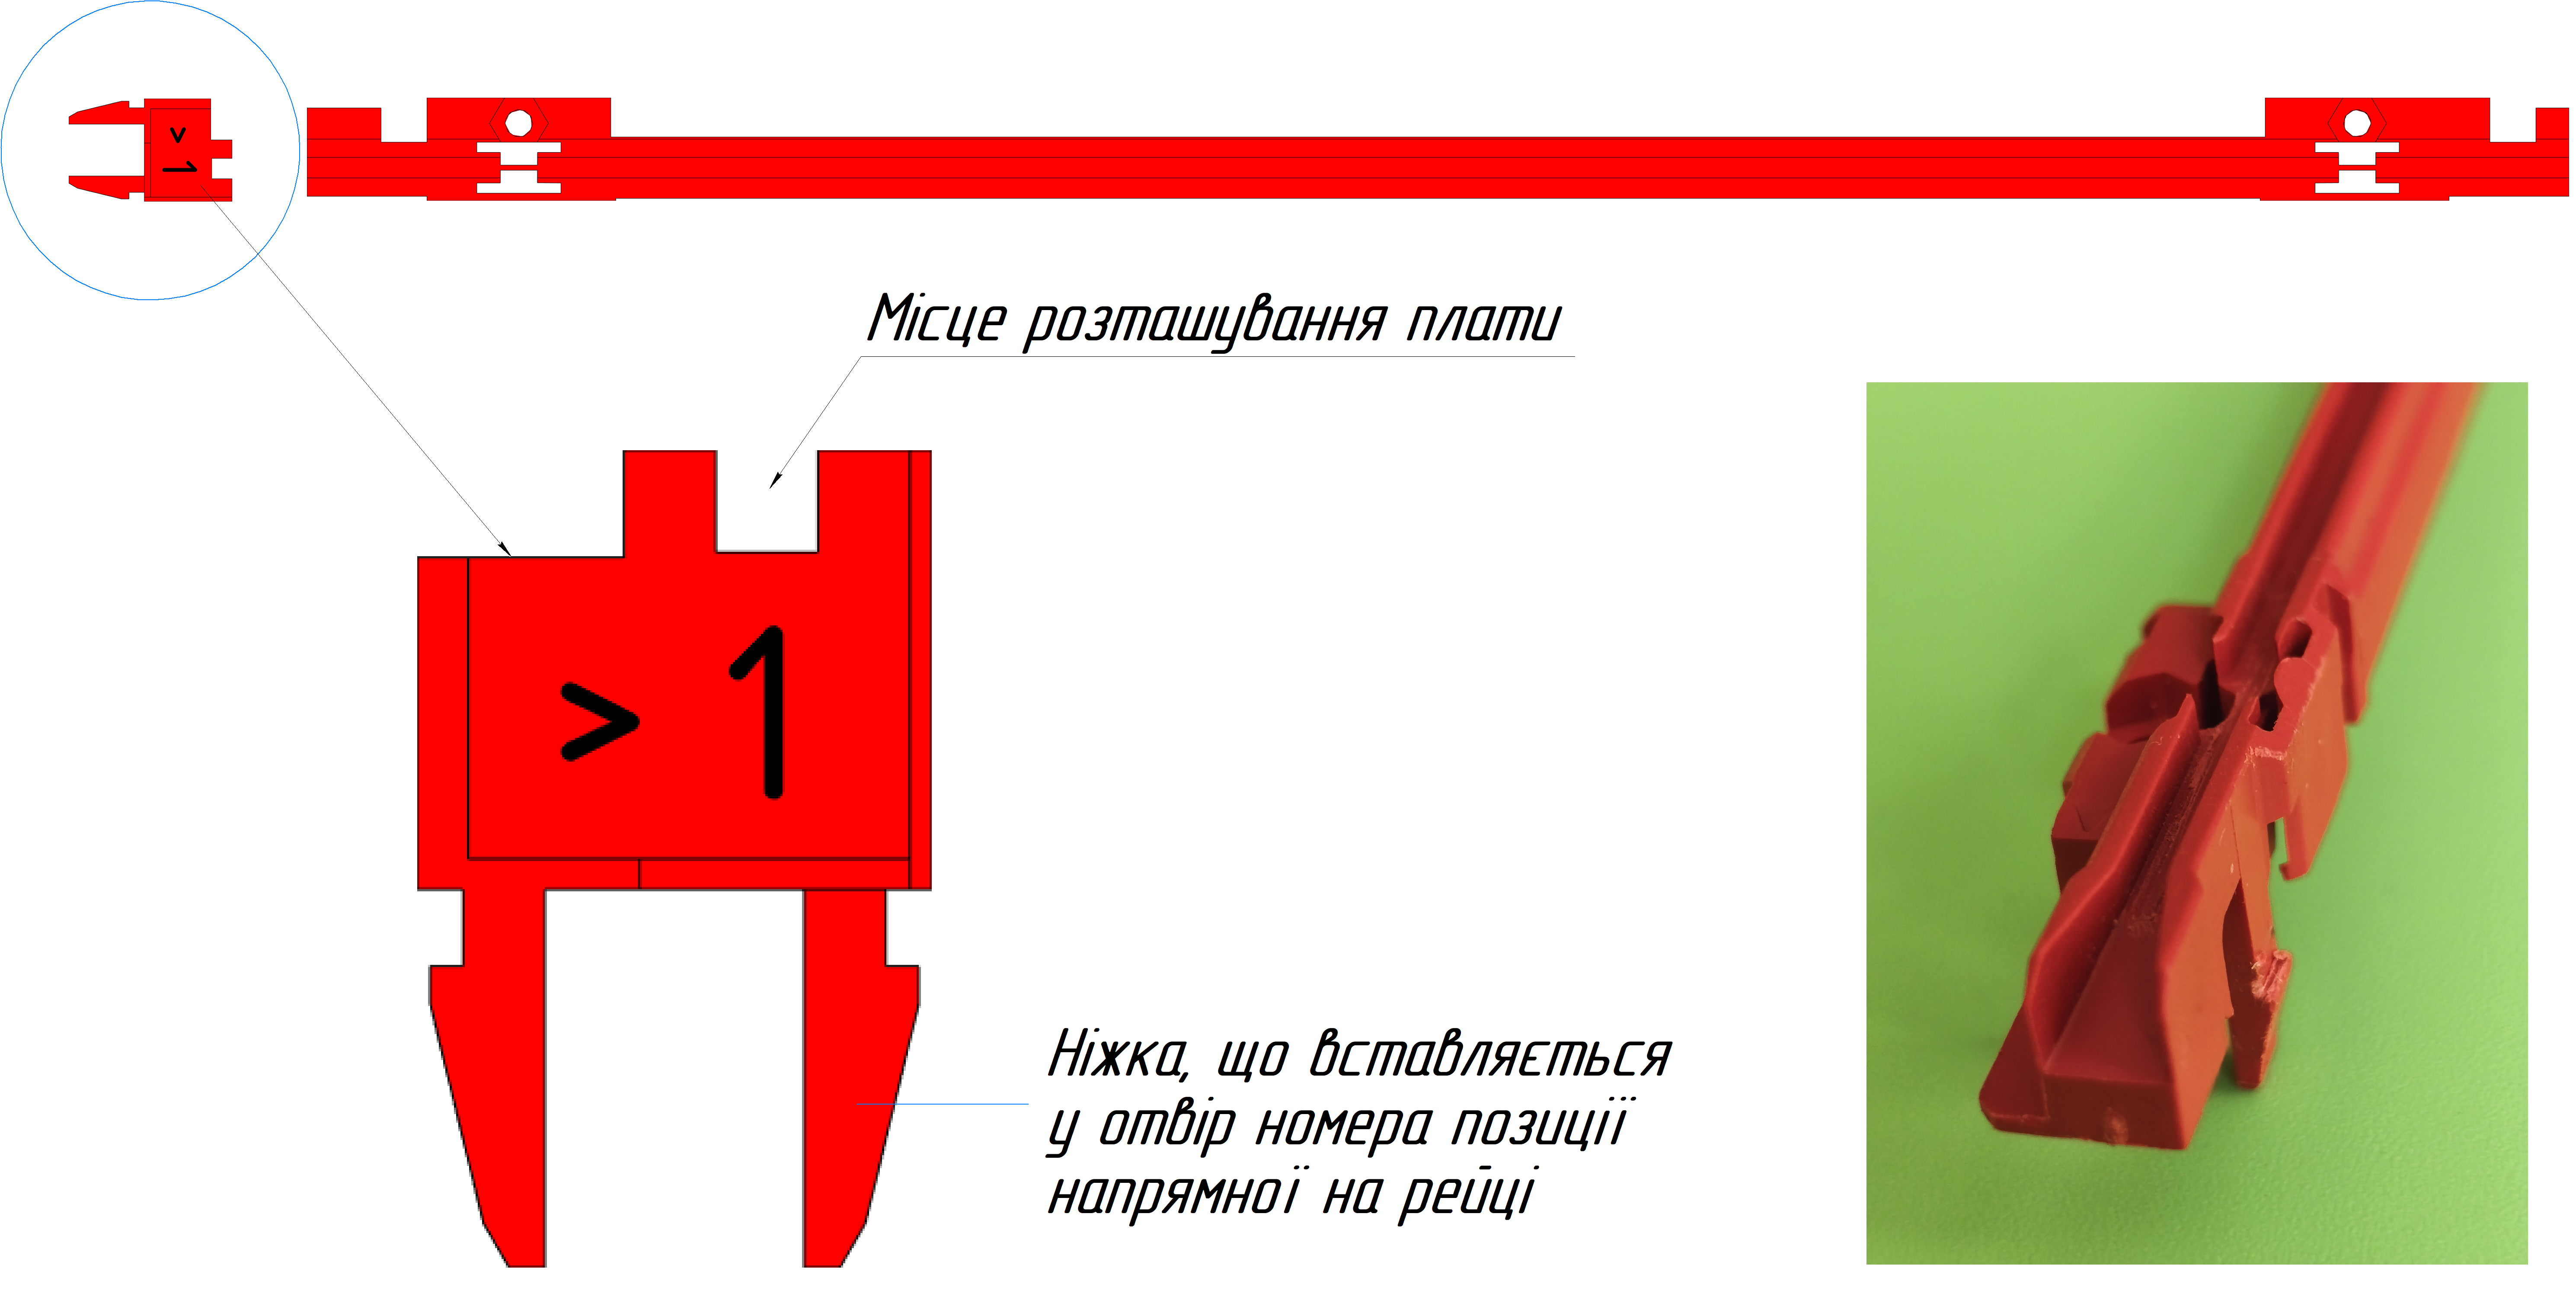
\includegraphics[width=1.0\textwidth]{images/A32.png} 
    \caption{Схема позиціонування напрямної при розміщенні на рейках}
\end{figure}

\newpage

% --- Підрозділ 3 ---
\section{Порядок складання}

Процес складання шасі має виконуватися в наступній послідовності:

\begin{enumerate}
    \item Встановити <<Планку контактну>>(Мал.1.11) на  <<Рейку передню L-KD>>(Мал.1.2) як вказано на Малюнку 1.24 у кількості 4(чотири) одиниці на один конструктив шасі.
\begin{figure}[H]
    \centering
    % Переконайтеся, що файл зображення завантажений в Overleaf
    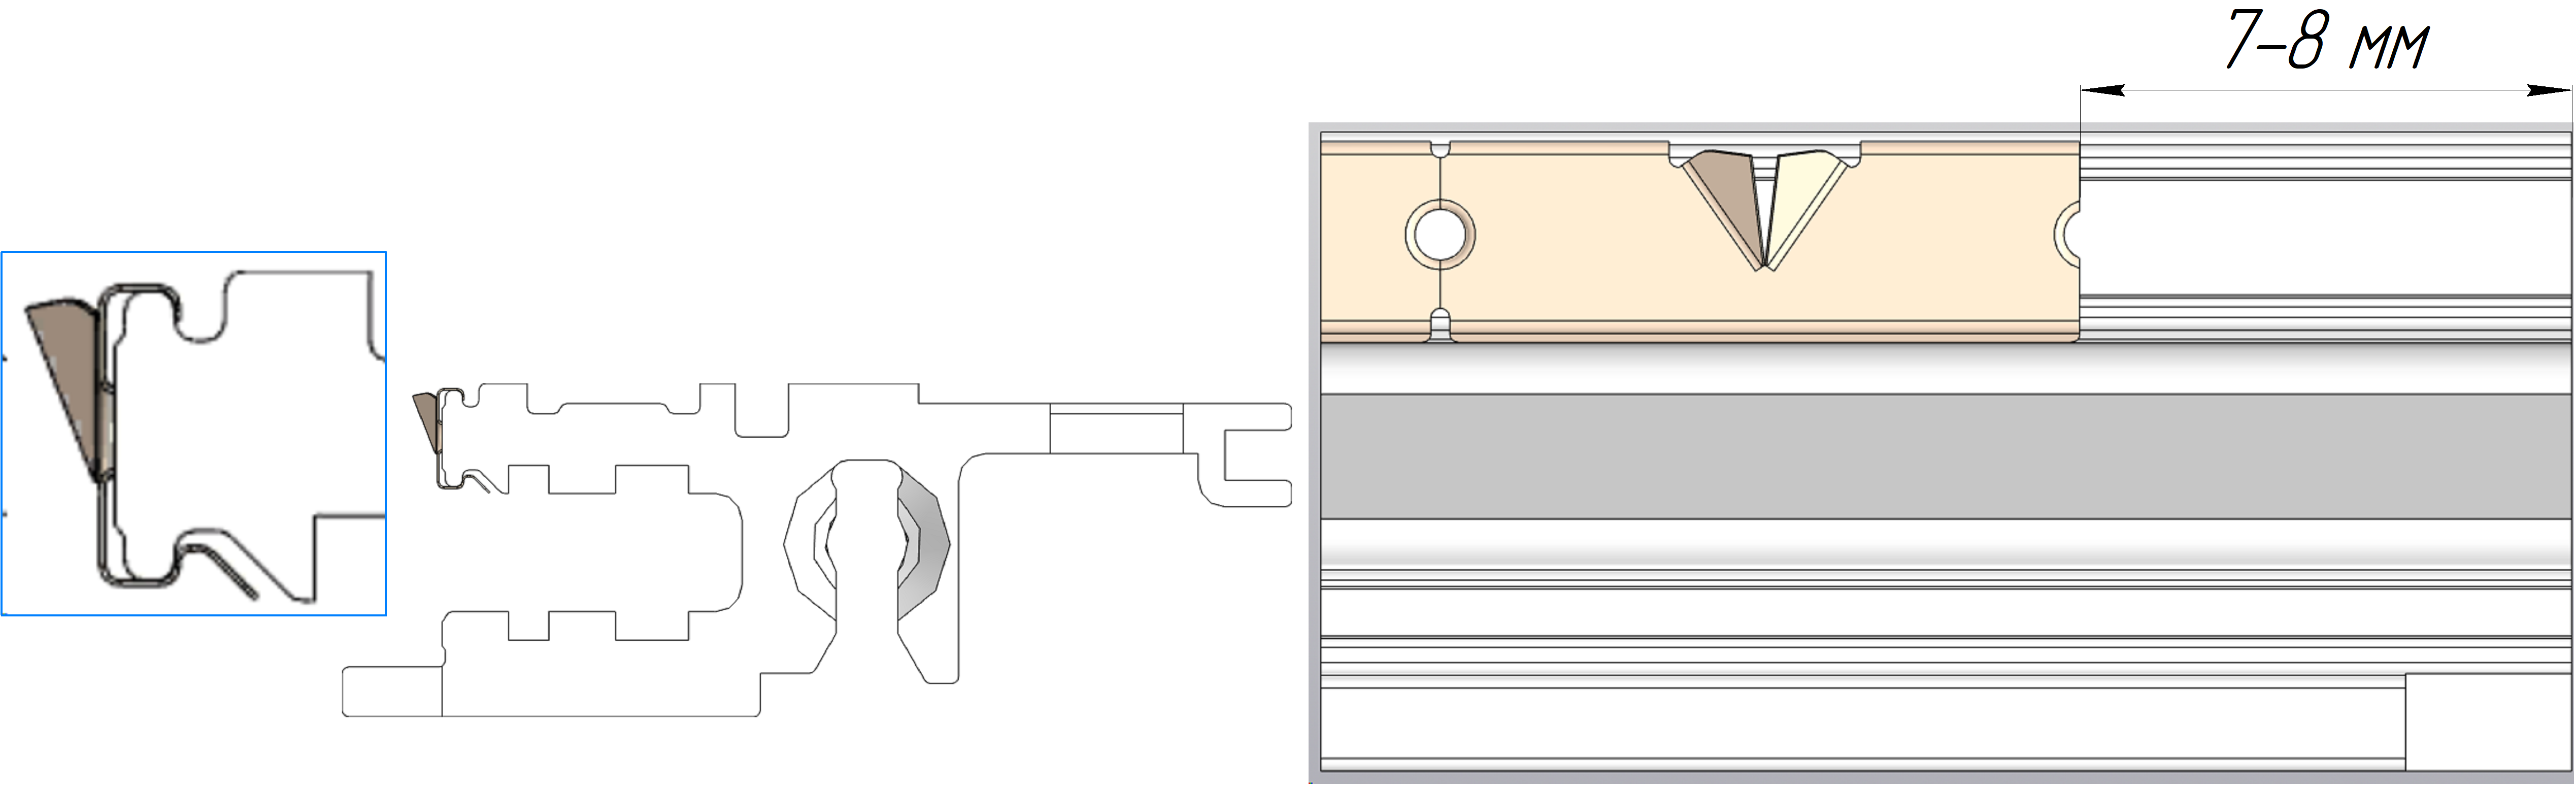
\includegraphics[width=0.7\textwidth]{images/A35.png} 
    \caption{Суміщення <<Рейки передньої L-KD>> та <<Планки контактної EuropacPRO EMC>> }
\end{figure}
    
    \item Вставити <<Планку різьбову М3х2х5 мм>> до відповідного поздовжнього пазу <<Рейки передньої L-KD>>(4 одиниці) та  <<Рейки задньої L-ST>>(2 одиниці) згідно з Малюнком 1.25.
\begin{figure}[H]
    \centering
    % Переконайтеся, що файл зображення завантажений в Overleaf
    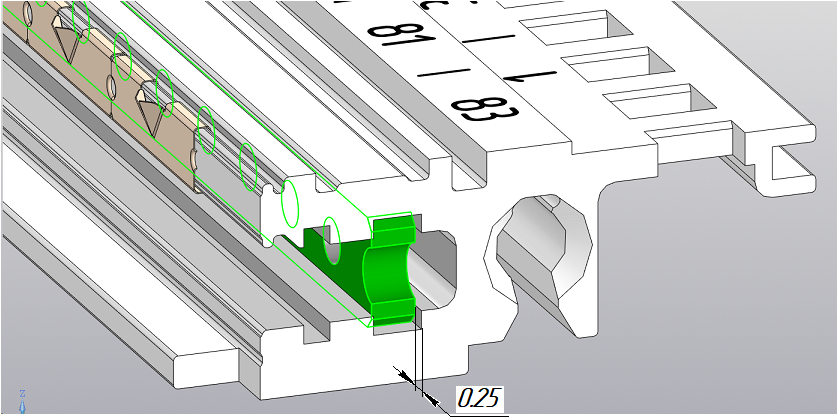
\includegraphics[width=0.6\textwidth]{images/A41.png} 
    \caption{Встановлення <<Планки різьбової М3х2х5мм>> до <<Рейки передньої L-KD>> та <<Рейки задньої L-ST>>}
\end{figure}
 
    \item Зафіксувати розташування <<Планки різьбової М3х2х5мм>>(Мал.1.10) за допомогою <<Фіксатора планки різьбової,М3х8 мм>>(Мал.1.12), дотримуючись вимог, що зображені на Малюнку 1.25. Відстань 0.25 мм між торцевими поверхнями <<Рейок>> та <<Планок>> позначена як орієнтовна. Вона дорівнює половині різниці длин <<Рейки передньої L-KD>> або <<Рейки задньої L-ST>> та <<Планки різьбової М3х2х5мм>>. Тобто ці деталі центруються відносно середини.

\begin{figure}[H]
    \centering
    % Переконайтеся, що файл зображення завантажений в Overleaf
    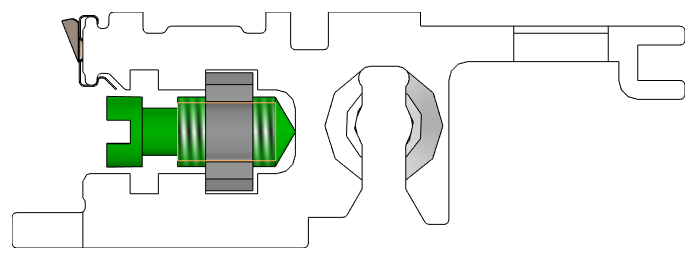
\includegraphics[width=0.6\textwidth]{images/A42.png} 
    \caption{Фіксація <<Планки різьбової М3х2х5мм>>}
\end{figure}

    \item Скласти бічні панелі(2 одиниці) конструктиву шасі як зображено на Малюнку 1.27.
\begin{figure}[H]
    \centering
    % Переконайтеся, що файл зображення завантажений в Overleaf
    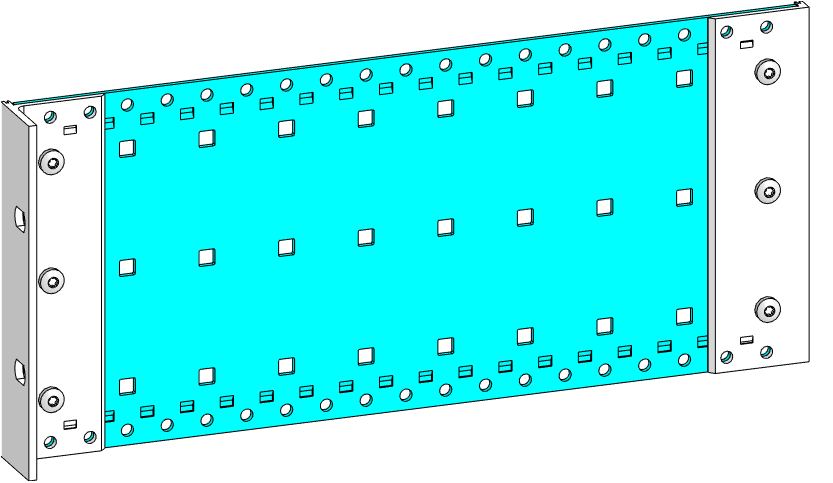
\includegraphics[width=0.5\textwidth]{images/A37.png} 
    \caption{Бічна панель конструктиву шасі}
\end{figure}
Для складання панелі треба використати <<Бічну панель EuropacPRO 3U19",295 мм.>>(Мал.1.1), <<Кронштейн EuropacPRO,3U>>(Мал.1.6), <<Профіль задній EuropacPRO,3U>>(Мал.1.7), <<Гайка квадратна, ступінчаста М4>>(Мал.1.15)(6 одиниць), <<Гвинт М4х6 мм, Torx>>(Мал.1.14)(6 одиниць).  
\begin{figure}[H]
    \centering
    % Переконайтеся, що файл зображення завантажений в Overleaf
    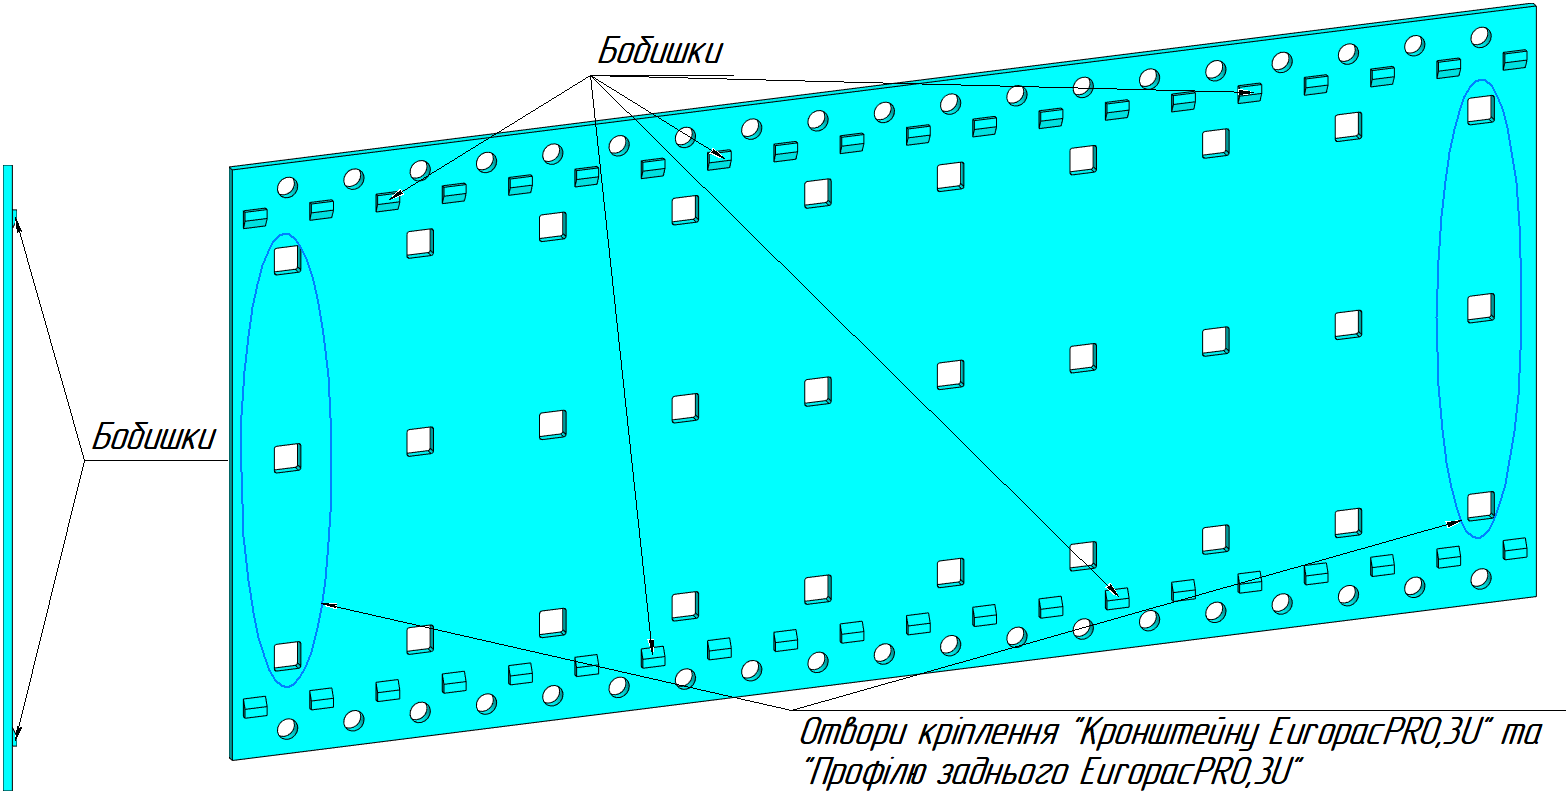
\includegraphics[width=0.7\textwidth]{images/A39.png} 
    \caption{Бічна панель EuropacPRO 3U19",295 мм.}
\end{figure}
Місця кріплення <<Кронштейну Europac PRO,3U>> та <<Профілю заднього Europac PRO,3U>> позначено на Малюнку 1.28. Симетрія <<Бічної панель Europac PRO 3U19",295 мм.>> не передбачає послідовності їх розміщення, тобто можно починати з будь якого краю. Кріплення здійснюється з використанням <<Гайок квадратних, ступінчастих, М4>> та <<Гвинтів М4х6 мм, Torx>>. Обидві деталі, тобто <<Кронштейн>> та <<Профіль>>, розташовуються на боці вільному від формованих бобишок(Мал.1.28), а <<Гайки>> вкладаються у квадратні отвори 6х6 мм з протилежного боку(з боку бобишок), послідовно по одній, з подальшим вкручуванням <<Гвинтів М4х6 мм, Torx>> з використанням динамометричної викрутки та біт Т15,Т20.  

\begin{mybox}{Важливо}
Момент затягування <<Гвинтів М4х6 мм, Torx>> має дорівнювати 2,4 Н*м. Використовувати битку T15,Т20 TORX.
\end{mybox}


    \item Встановити на одну із складених бічних панелей(Мал.1.27) <<Гвинт заземлення>>, як зображено на Малюнку 1.29, використовуючи <<Гайку квадратну, ступінчасту М4>>(Мал.1.15), <<Шайбу 4 стопорну A4 із зовнішніми зубцями>>(мал.1.19) та <<Гвинт М4х16 бурт. 10.9 цб INB>>(Мал.1.20). Гвинт вкручується з використанням динамометричної викрутки та біти HEX2.5.
\begin{figure}[H]
    \centering
    % Переконайтеся, що файл зображення завантажений в Overleaf
    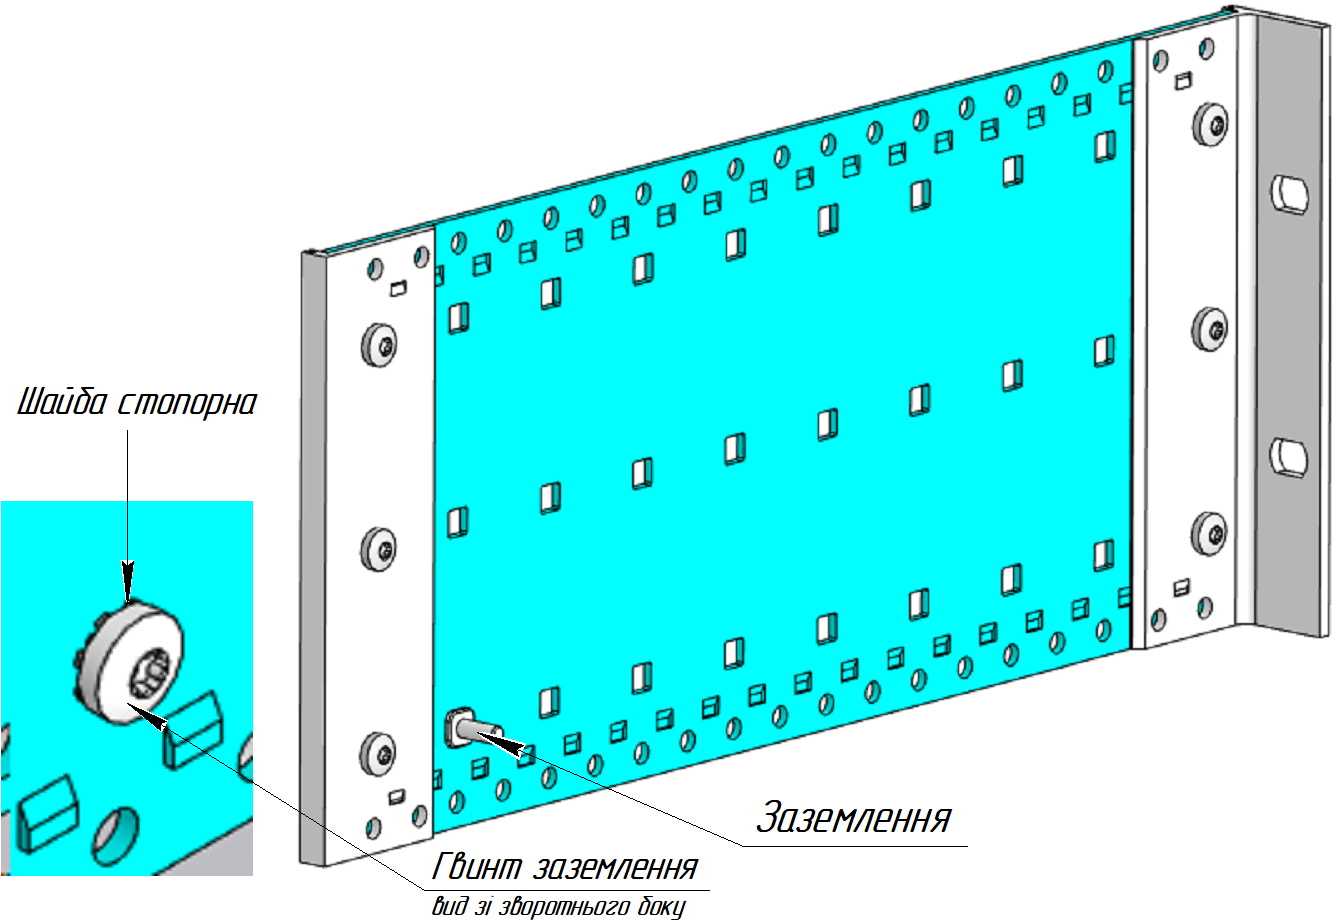
\includegraphics[width=0.5\textwidth]{images/A43.png} 
    \caption{Права бічна панель конструктиву шасі}
\end{figure}
\begin{mybox}{Важливо}
Момент затягування <<Гвинта М4х16 бурт. 10.9 цб INB>> має дорівнювати 1,8-1.9 Н*м. Використовувати біту HEX2.5.
\end{mybox}
Треба звернути увагу, що після розміщення <<Гвинта заземлення>> ця <<Бічна пенель>> набуває статус <<Права бічна панель>> конструктиву шасі, а інша стає  <<Лівою бічною панеллю>> згідно схеми, що зображена на Малюнку 1.20

    \item Скласти нижню частину конструктиву шасі, як зображено на Малюнку 1.30.
    \centering
     Переконайтеся, що файл зображення завантажений в Overleaf
    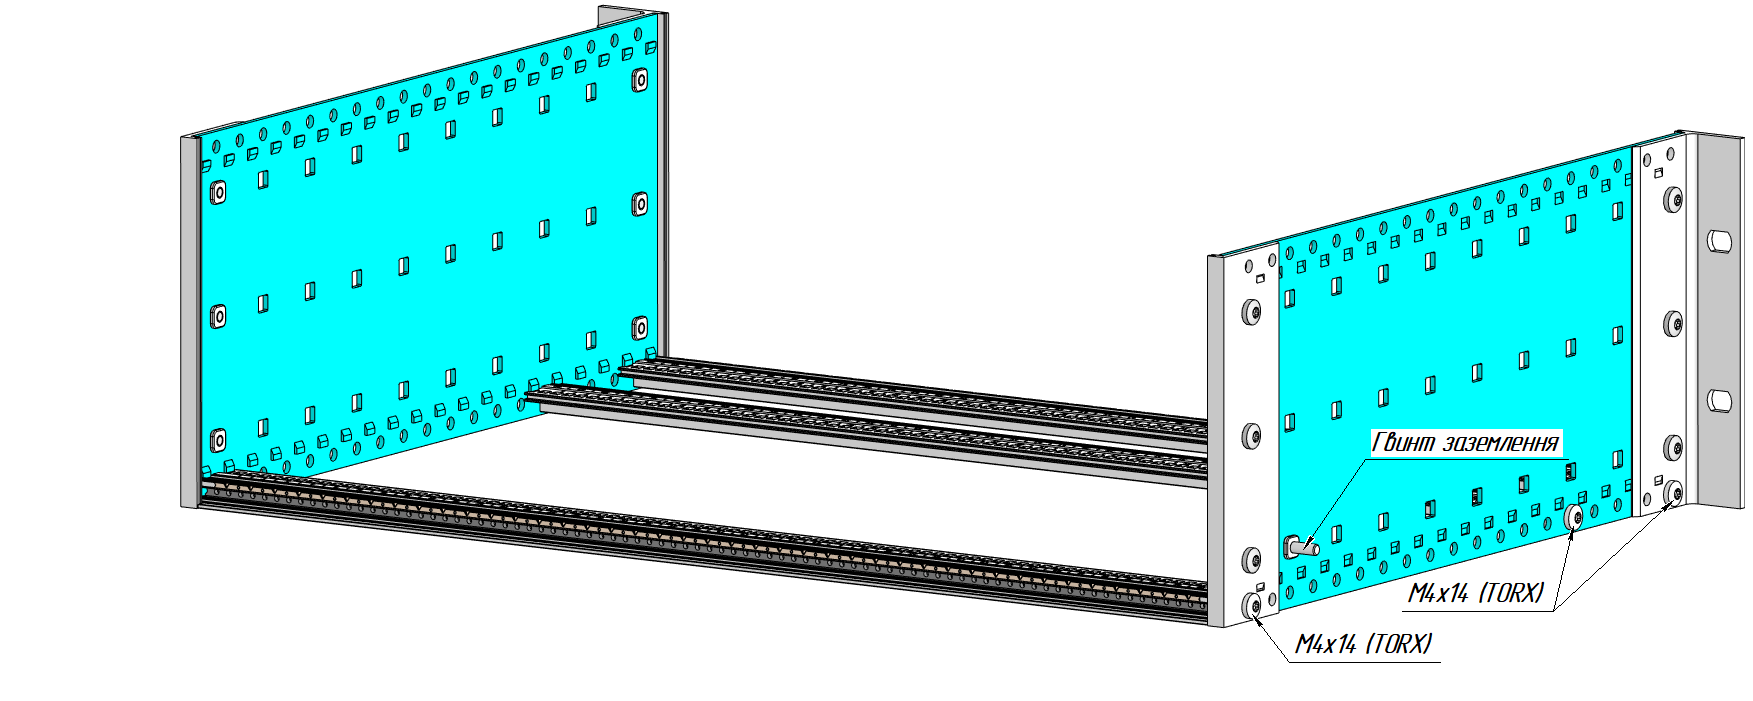
\includegraphics[width=0.5\textwidth]{images/A46.png} 
    \caption{Нижня частина конструктиву шасі}
\end{figure}




\end{enumerate}



\begin{mybox}{Важливо}
Момент затягування гвинтів М4х14 кріплення рейок <<L-KD>> та <<L-ST>> має дорівнюватися 2,4 Н*м.
Теж саме для гвинтів М4х6 кріплення <<Кронштейну>>(24560-197) та <<Профілю заднього"(24561-198).
Момент затягування квинтів М4х6 кріплення верхньої та нижньої панелей має дорівнювати 1,8 Н*м.
\end{mybox}

\newpage

% --- Підрозділ 4 ---
\section{Особливості розміщення екранів}
При встановленні екранованих панелей необхідно звернути увагу на забезпечення надійного електричного контакту з корпусом.

\begin{figure}[H]
    \centering
    % Переконайтеся, що файл зображення завантажений в Overleaf
    
\includegraphics[width=1.0\textwidth]{images/A27.pdf} 
    \caption{Схема розміщення екрануючих елементів}
\end{figure}

\begin{mybox}{Важливо}
Не допускайте потрапляння фарби на місця контакту екранів з шинами заземлення.
\end{mybox}
